\documentclass[11pt,a4paper]{article}

\usepackage[utf8]{inputenc}
\usepackage[T1]{fontenc}
\usepackage[spanish,es-noshorthands,es-nodecimaldot]{babel}
\usepackage{lmodern}
\usepackage[margin=2.3cm]{geometry}
\usepackage{amsmath,amssymb}
\usepackage{graphicx}
\usepackage{xcolor}
\usepackage{booktabs}
\usepackage{array}
\usepackage{tabularx}
\usepackage{float}
\usepackage{caption}
\usepackage{enumitem}
\usepackage{fancyhdr}
\usepackage[hidelinks]{hyperref}

% ---------------------------------------------------------------
% Marcas de pendientes (en ROJO). Buscar "\pendiente" para ubicarlas.
% ---------------------------------------------------------------
\newcommand{\pendiente}[1]{\textcolor{red}{\textbf{[PENDIENTE: #1]}}}
\newcommand{\fotopendiente}[1]{%
  \begin{center}
    \fcolorbox{red}{red!5}{\parbox{0.8\linewidth}{\centering\vspace{1.2cm}
      \textcolor{red}{\textbf{[PENDIENTE: FOTO]}}\\[2pt]\textcolor{red}{#1}\vspace{1.2cm}}}
  \end{center}}

\captionsetup{font=small,labelfont=bf}
\setlist{itemsep=2pt}
\renewcommand{\arraystretch}{1.25}

\pagestyle{fancy}
\setlength{\headheight}{14pt}
\fancyhf{}
\lhead{\small Óptica y Ondas -- Laboratorio 2}
\rhead{\small Universidad de Ingeniería y Tecnología}
\cfoot{\thepage}

\begin{document}

% =========================================================
% PORTADA
% =========================================================
\hypersetup{pageanchor=false}
\begin{titlepage}
\thispagestyle{empty}
\definecolor{morado}{HTML}{7030A0}
\begin{center}
    
\includegraphics[width=0.50\textwidth]{imagenes/logo.jpeg}\\[0.3cm]

    {\Large\bfseries CC1123 - Óptica y Ondas\par}
    {\large Teoría 1\par}
    \vspace{0.6cm}

    {\fontsize{24}{28}\selectfont\bfseries\color{morado} Laboratorio 2\par}
    \vspace{0.35cm}
    {\Large\bfseries Formación y análisis de imágenes en\\ espejos cóncavos y convexos\par}
    \vspace{1cm}

    {\large\textbf{Profesor:}\par}
    \vspace{0.2cm}
    Cuyubamba Espinoza, Marco Antonio\par
    \vspace{0.5cm}

    {\large\textbf{Integrantes:}\par}
    \vspace{0.2cm}
    Chirinos Zelada, Ricardo Raimundo\par
    Docarmo Rodriguez, Luis Jaime\par
    Escalante Ccoyllo, Nahía Alejandra\par
    Gutierrez Soto, Brhandon Luis\par
    \vspace{0.5cm}

    {\large\textbf{Fecha:}\par}
    \vspace{0.2cm}
    8 de noviembre de 2026\par
\end{center}
\end{titlepage}
\hypersetup{pageanchor=true}

% ---------------------------------------------------------------
\begin{center}
\fcolorbox{red}{red!3}{\parbox{0.92\linewidth}{
\textcolor{red}{\textbf{LISTA DE PENDIENTES (borrar este recuadro antes de entregar)}}
\begin{enumerate}[leftmargin=*]
  \item \textcolor{red}{Enlace del video de YouTube (máx.\ 10 min).}
  \item \textcolor{red}{Enlace a los datos experimentales y a los scripts.}
\end{enumerate}}}
\end{center}

% ---------------------------------------------------------------
\section*{Enlaces}
\begin{itemize}
  \item \textbf{Video explicativo (YouTube, máx.\ 10 min):} \pendiente{enlace de YouTube}
  \item \textbf{Datos experimentales y cálculos:} \pendiente{enlace a la carpeta con los datos y los scripts de \texttt{figuras/}}
\end{itemize}

% ===============================================================
\section{Introducción}

\subsection{Objetivos}
\begin{enumerate}
  \item Analizar las características de las imágenes formadas por un espejo cóncavo.
  \item Calcular experimentalmente la distancia focal $f$ y el radio de curvatura $R$ de un espejo cóncavo.
  \item Distinguir experimentalmente entre un espejo cóncavo y uno convexo.
\end{enumerate}

\subsection{Conclusión principal}
Tres métodos dan valores compatibles de la distancia focal: $f = 19.18 \pm 0.05$~cm (ecuación del espejo), $18.9 \pm 1.5$~cm (ajuste de $M$ vs $d_i$) y $19.25 \pm 0.67$~cm (recta de inversas), es decir, $R \approx 38$~cm (nominal: $f = 20$~cm). El cóncavo forma imágenes reales e invertidas para $d_o > f$; el convexo nunca forma una imagen proyectable.

\subsection{Palabras clave}
Espejo esférico (cóncavo y convexo) $\cdot$ Radio de curvatura $\cdot$ Distancia focal $\cdot$ Imagen real y virtual $\cdot$ Imagen derecha o invertida $\cdot$ Distancia objeto y distancia imagen $\cdot$ Factor de magnificación $\cdot$ Trazado de rayos $\cdot$ Rayo paralelo, focal, radial y central.

% ===============================================================
\section{Fundamento teórico}

Un espejo esférico es una sección de esfera con centro de curvatura $C$ y vértice $S$. La distancia entre ambos es el radio de curvatura $R$, y el foco $F$ está a la mitad:
\begin{equation}
  f = \frac{R}{2}
\end{equation}
La posición de la imagen la da la ecuación del espejo:
\begin{equation}
  \frac{1}{d_o} + \frac{1}{d_i} = \frac{1}{f} \quad \Longleftrightarrow \quad d_i = \frac{d_o f}{d_o - f}
  \label{eq:espejo}
\end{equation}
y su tamaño, el factor de magnificación:
\begin{equation}
  M = \frac{h_i}{h_o} = -\frac{d_i}{d_o}
  \label{eq:aumento}
\end{equation}
Combinando \eqref{eq:espejo} y \eqref{eq:aumento} se obtienen las dos rectas del análisis:
\begin{equation}
  M = 1 - \frac{d_i}{f} \qquad \Longrightarrow \qquad |M| = \frac{1}{f}\,d_i - 1 \quad (\text{imagen real e invertida})
  \label{eq:lineal}
\end{equation}
y, con las inversas de las distancias, una recta de pendiente $-1$ que corta el eje vertical en $1/f$:
\begin{equation}
  \frac{1}{d_o} = -\frac{1}{d_i} + \frac{1}{f}
  \label{eq:inversas}
\end{equation}

\paragraph{Convención de signos} (Apéndice D.3 de la guía):
\begin{center}
\begin{tabular}{lll}
\toprule
\textbf{Variable} & \textbf{Condición} & \textbf{Signo} \\
\midrule
Distancia focal $f$ & Espejo cóncavo / convexo & $+$ / $-$ \\
Distancia objeto $d_o$ & En todo el experimento & $+$ \\
Distancia imagen $d_i$ & Imagen real / virtual & $+$ / $-$ \\
Magnificación $M$ & Imagen derecha / invertida & $+$ / $-$ \\
\bottomrule
\end{tabular}
\end{center}

\paragraph{Rayos para el trazado.} (1) Rayo paralelo: llega paralelo al eje y se refleja pasando por $F$ (en el convexo, parece venir de $F$). (2) Rayo focal: pasa por $F$ y se refleja paralelo al eje. (3) Rayo radial: pasa por $C$ y regresa sobre sí mismo. (4) Rayo central: incide en el vértice y se refleja simétricamente respecto al eje.

% ===============================================================
\section{Métodos}

\subsection{Equipo}
\begin{enumerate}
  \item Riel óptico graduado.
  \item Fuente de luz con flecha (objeto de altura $h_o = 2$~cm).
  \item Soporte para pantalla, con una tira gruesa de hoja Bond como pantalla.
  \item Soportes deslizantes.
  \item Espejo cóncavo-convexo de doble cara ($f$ nominal $= 20$~cm).
  \item Regla de 30~cm, hojas Bond y plumón.
\end{enumerate}
El arreglo montado se muestra en la Figura~\ref{fig:montaje}.

\begin{figure}[H]
  \centering
  \begin{minipage}{0.48\linewidth}\centering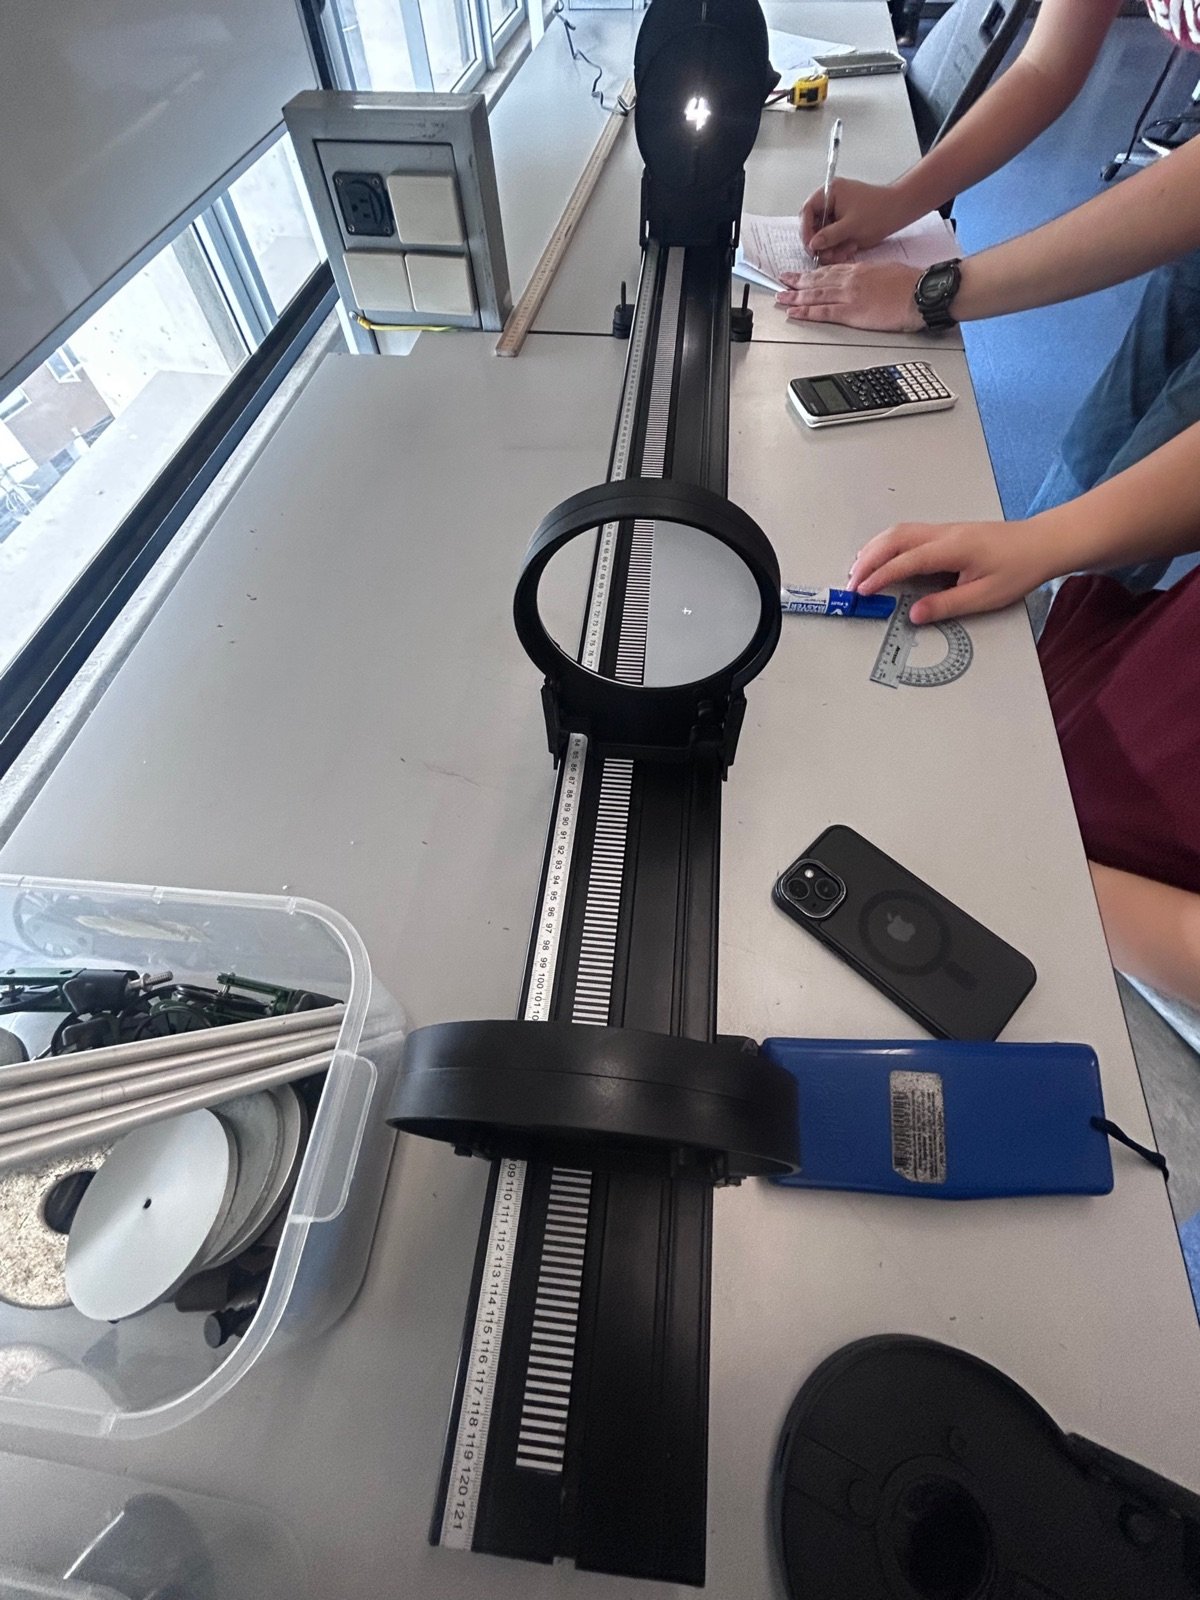
\includegraphics[height=7.5cm,width=\linewidth,keepaspectratio]{fotos/lab/04.jpg}\\[2pt]\small (a)\end{minipage}\hfill
  \begin{minipage}{0.48\linewidth}\centering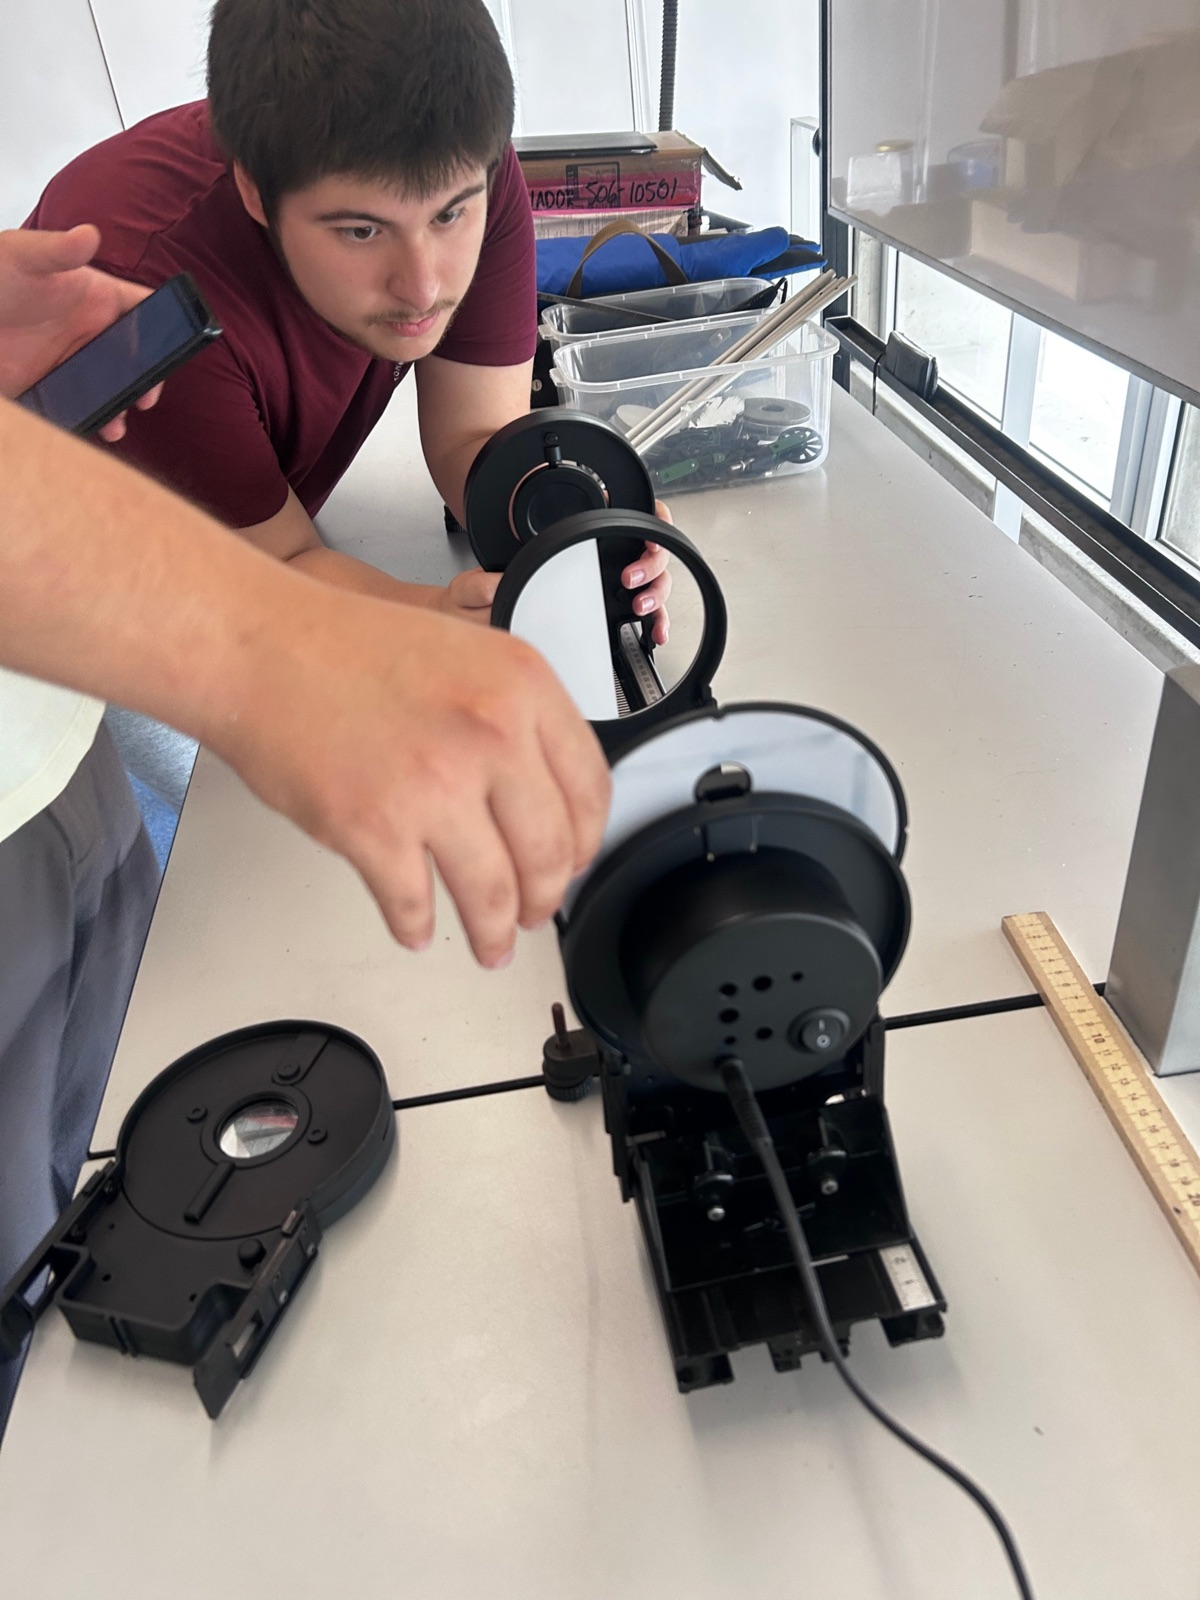
\includegraphics[height=7.5cm,width=\linewidth,keepaspectratio]{fotos/lab/01.jpg}\\[2pt]\small (b)\end{minipage}
  \caption{Arreglo experimental. (a) Vista a lo largo del riel: la fuente con la flecha al fondo, la pantalla en el centro y el espejo en primer plano. (b) Fuente de luz, pantalla y espejo cóncavo en sus soportes; a la izquierda, el espejo convexo.}
  \label{fig:montaje}
\end{figure}

\subsection{Procedimiento}

\paragraph{Trazado de rayos (antes del experimento).}
\begin{enumerate}
  \item Espejo cóncavo (Apéndice A): diagramas para $d_o = f$, $d_o > R$, $d_o = R$, $f < d_o < R$ y $d_o < f$.
  \item Espejo convexo (Apéndice B): diagramas para $d_o > R$, $f < d_o < R$ y $d_o < f$.
\end{enumerate}

\paragraph{Determinación de $f$ y $R$ (Cuadro~\ref{tab:datos}).}
\begin{enumerate}[resume]
  \item Se montaron la fuente, el soporte de pantalla y el espejo en el riel, con la cara cóncava hacia la fuente.
  \item Se dobló una tira de hoja Bond hasta formar una pantalla gruesa y compacta, y se colocó en su soporte.
  \item El objeto (la flecha) quedó en la marca de 8~cm del riel, así que $d_o$ es la lectura del espejo menos 8~cm (p.\ ej., $57.2 - 8 = 49.2$~cm). Se midió $h_o = 2$~cm.
  \item Se fijó el espejo a una distancia $d_o$ y se movió la pantalla hasta obtener la imagen más nítida (Figura~\ref{fig:enfoque}). Se registraron $d_o$ y $d_i$ en la hoja de datos (Figura~\ref{fig:registro}).
  \item Sin mover la pantalla, se marcaron los extremos de la imagen con plumón y se midió $h_i$ con la regla.
  \item Se repitió para seis $d_o$ cada 5~cm (49.2 a 74.2~cm) y un caso extremo a propósito, $d_o = 99.2$~cm.
\end{enumerate}

\begin{figure}[H]
  \centering
  \begin{minipage}{0.48\linewidth}\centering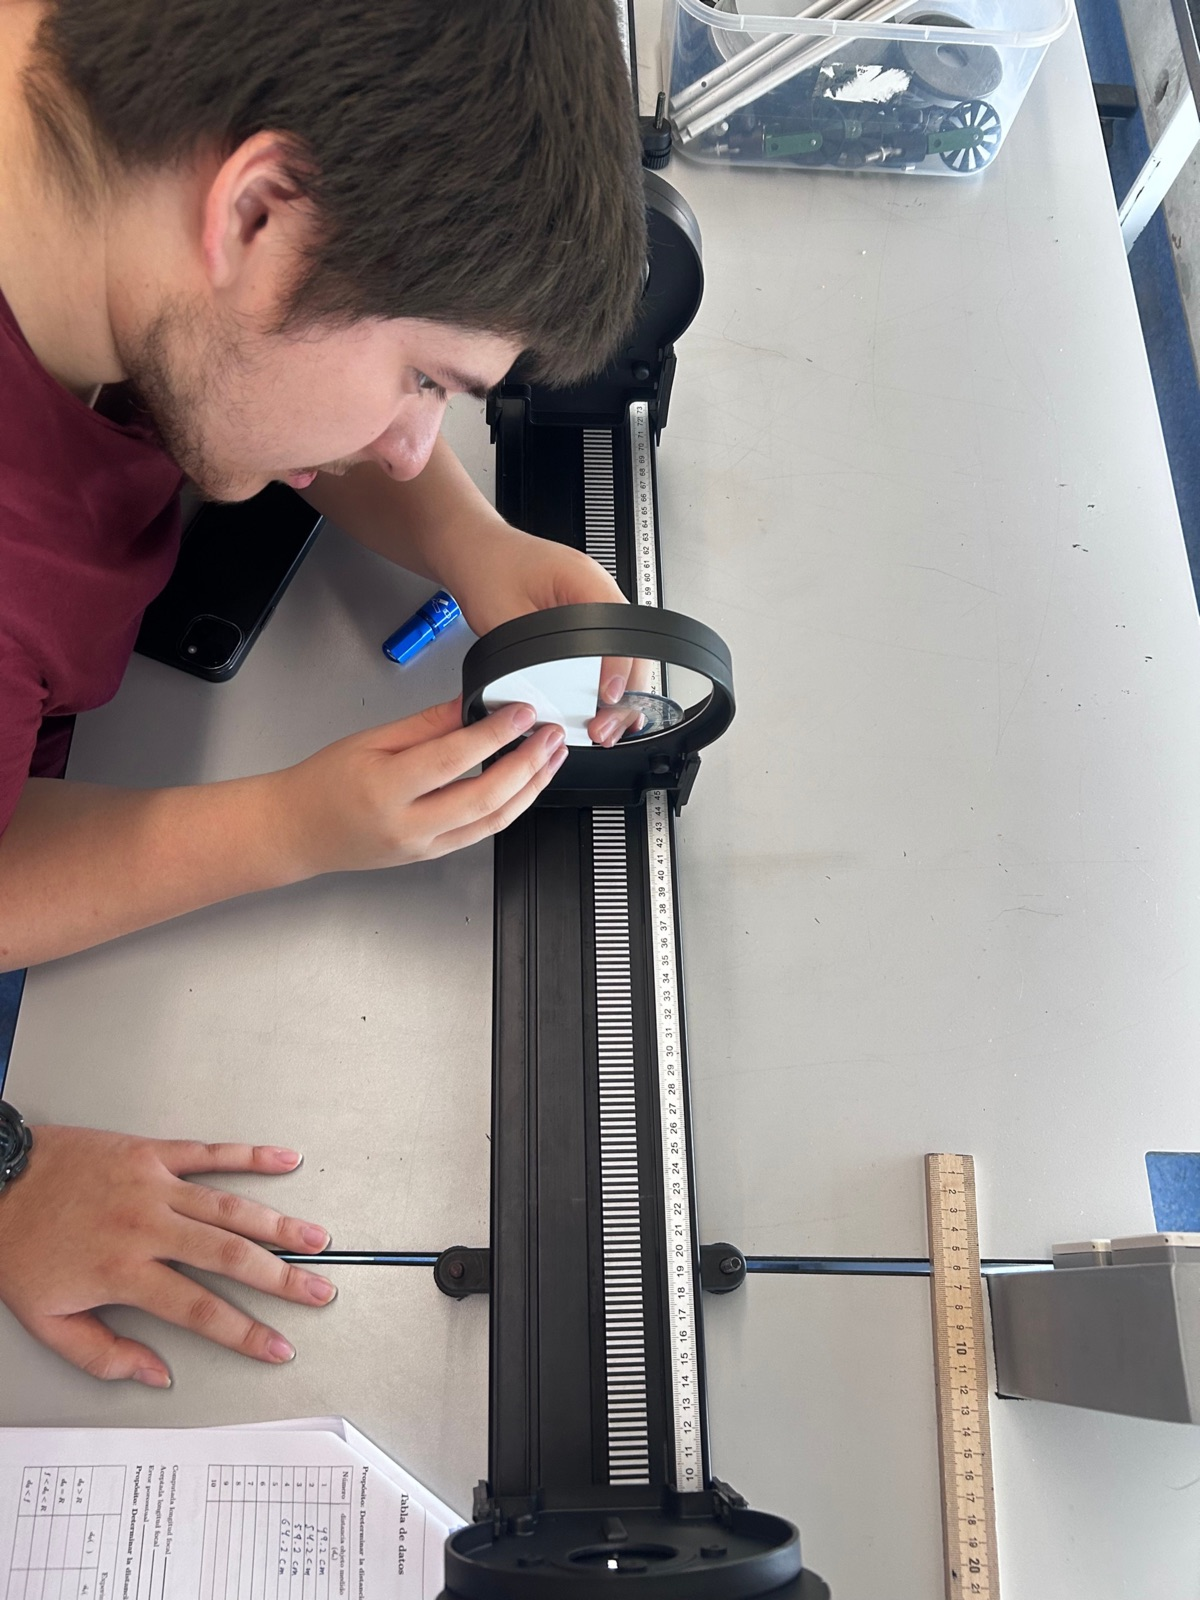
\includegraphics[height=7.5cm,width=\linewidth,keepaspectratio]{fotos/lab/02.jpg}\\[2pt]\small (a)\end{minipage}\hfill
  \begin{minipage}{0.48\linewidth}\centering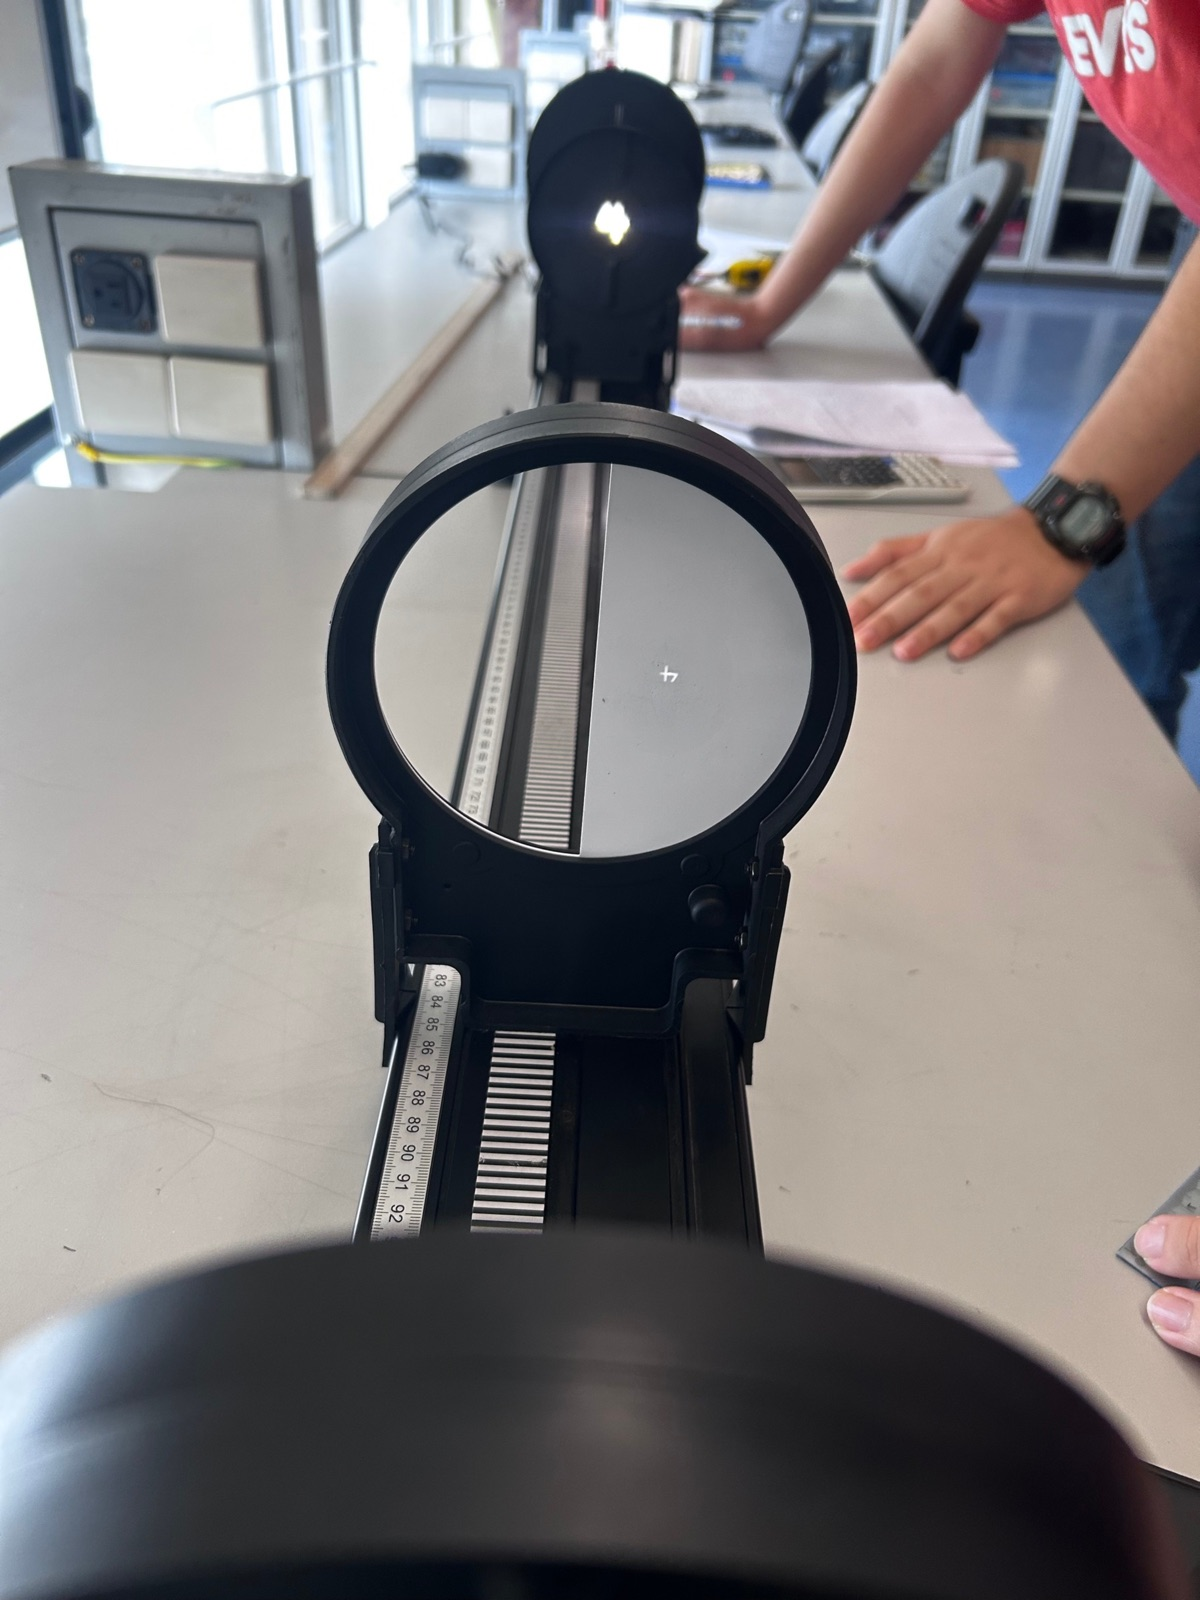
\includegraphics[height=7.5cm,width=\linewidth,keepaspectratio]{fotos/lab/05.jpg}\\[2pt]\small (b)\end{minipage}
  \caption{(a) Búsqueda de la imagen nítida desplazando la pantalla sobre el riel. (b) Imagen enfocada en la pantalla, vista desde detrás del espejo: real, invertida y reducida respecto a la flecha de la fuente.}
  \label{fig:enfoque}
\end{figure}
\begin{figure}[H]
  \centering
  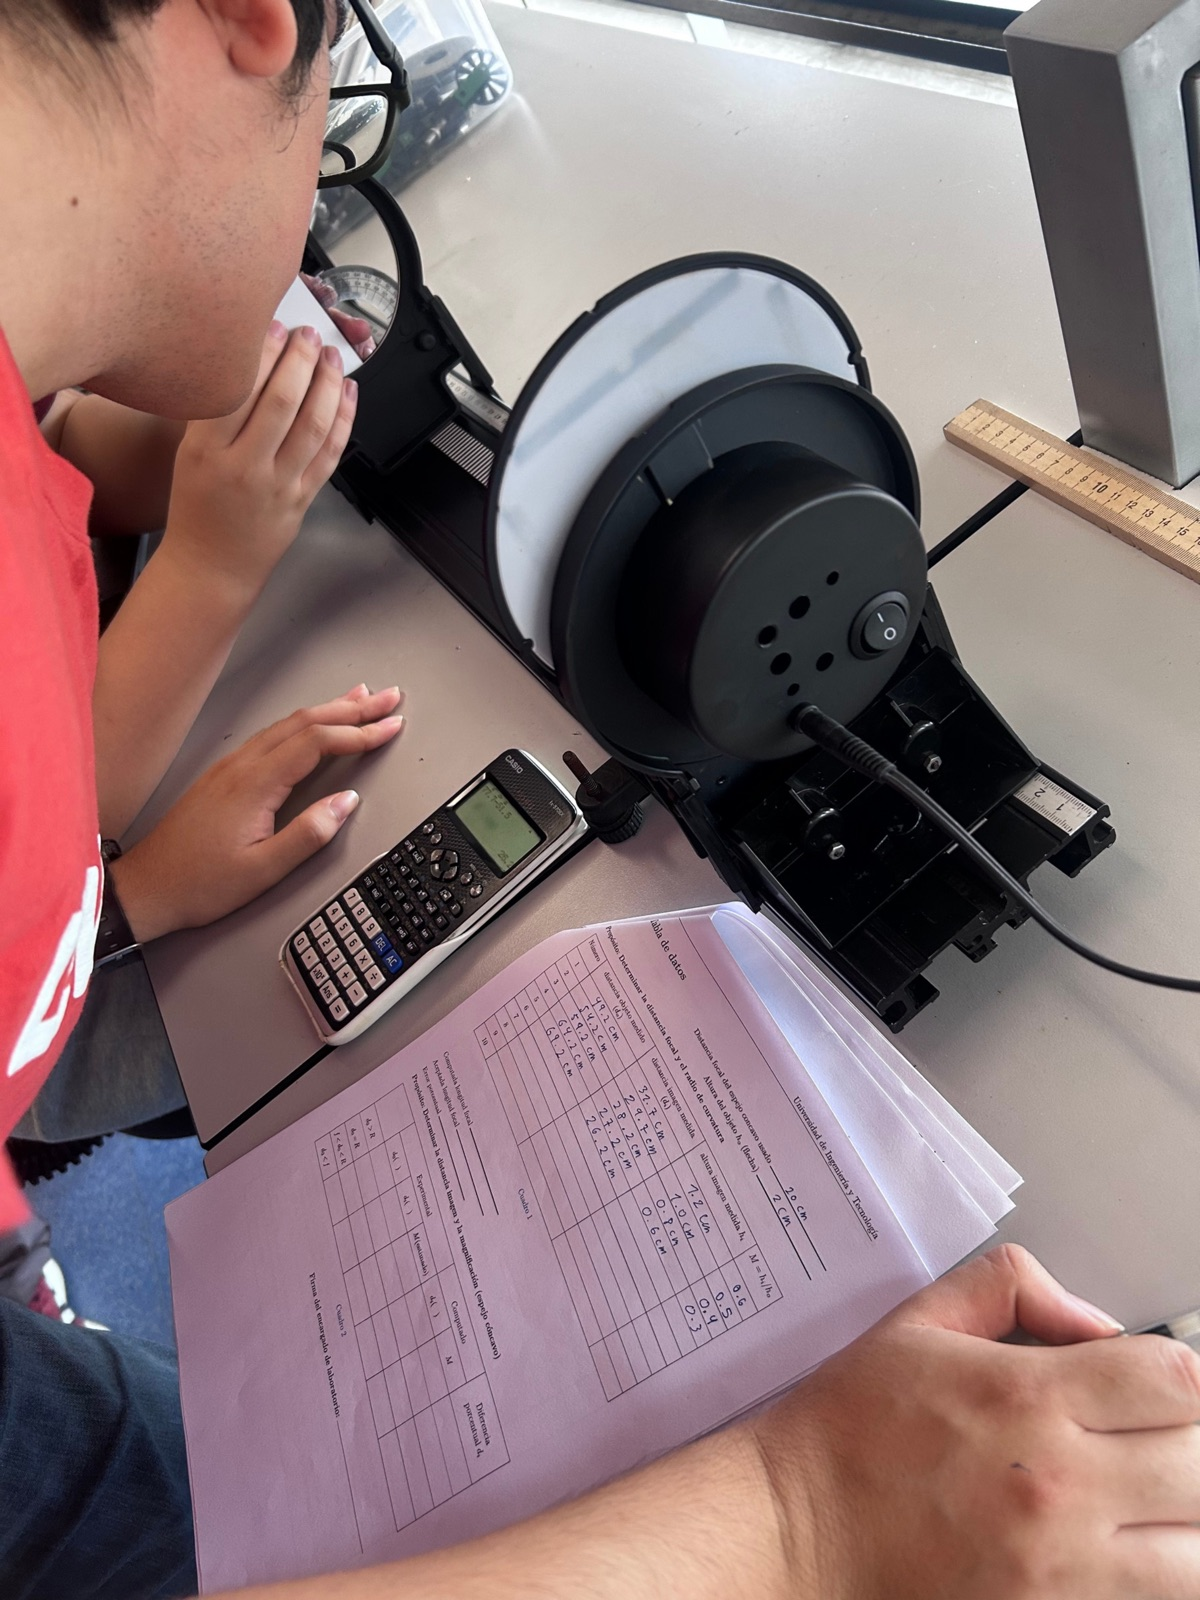
\includegraphics[height=7.5cm]{fotos/lab/03.jpg}
  \caption{Registro de $d_o$, $d_i$ y $h_i$ en la hoja de datos (Cuadro~\ref{tab:datos}) durante la medición.}
  \label{fig:registro}
\end{figure}

\paragraph{Casos del espejo cóncavo (Cuadro~\ref{tab:casos}).}
\begin{enumerate}[resume]
  \item Se colocó el objeto en $d_o > R$ (45~cm), $d_o = R$ (40~cm), $f < d_o < R$ (35~cm) y $d_o < f$ (15~cm). Aquí $d_o$ se midió directamente con la regla, de la flecha al espejo (por eso son valores enteros, a diferencia del Cuadro~\ref{tab:datos}). En cada caso se midió $d_i$, se estimó $M = -d_i/d_o$ (sin medir alturas, como indica la guía) y se comparó $d_i$ con el valor de la ecuación~\eqref{eq:espejo}.
\end{enumerate}

\paragraph{Espejo convexo.}
\begin{enumerate}[resume]
  \item Con la cara convexa y el objeto a una distancia arbitraria, se buscó la imagen moviendo la pantalla por el riel; luego se miró directamente el espejo.
\end{enumerate}

\begin{figure}[H]
  \centering
  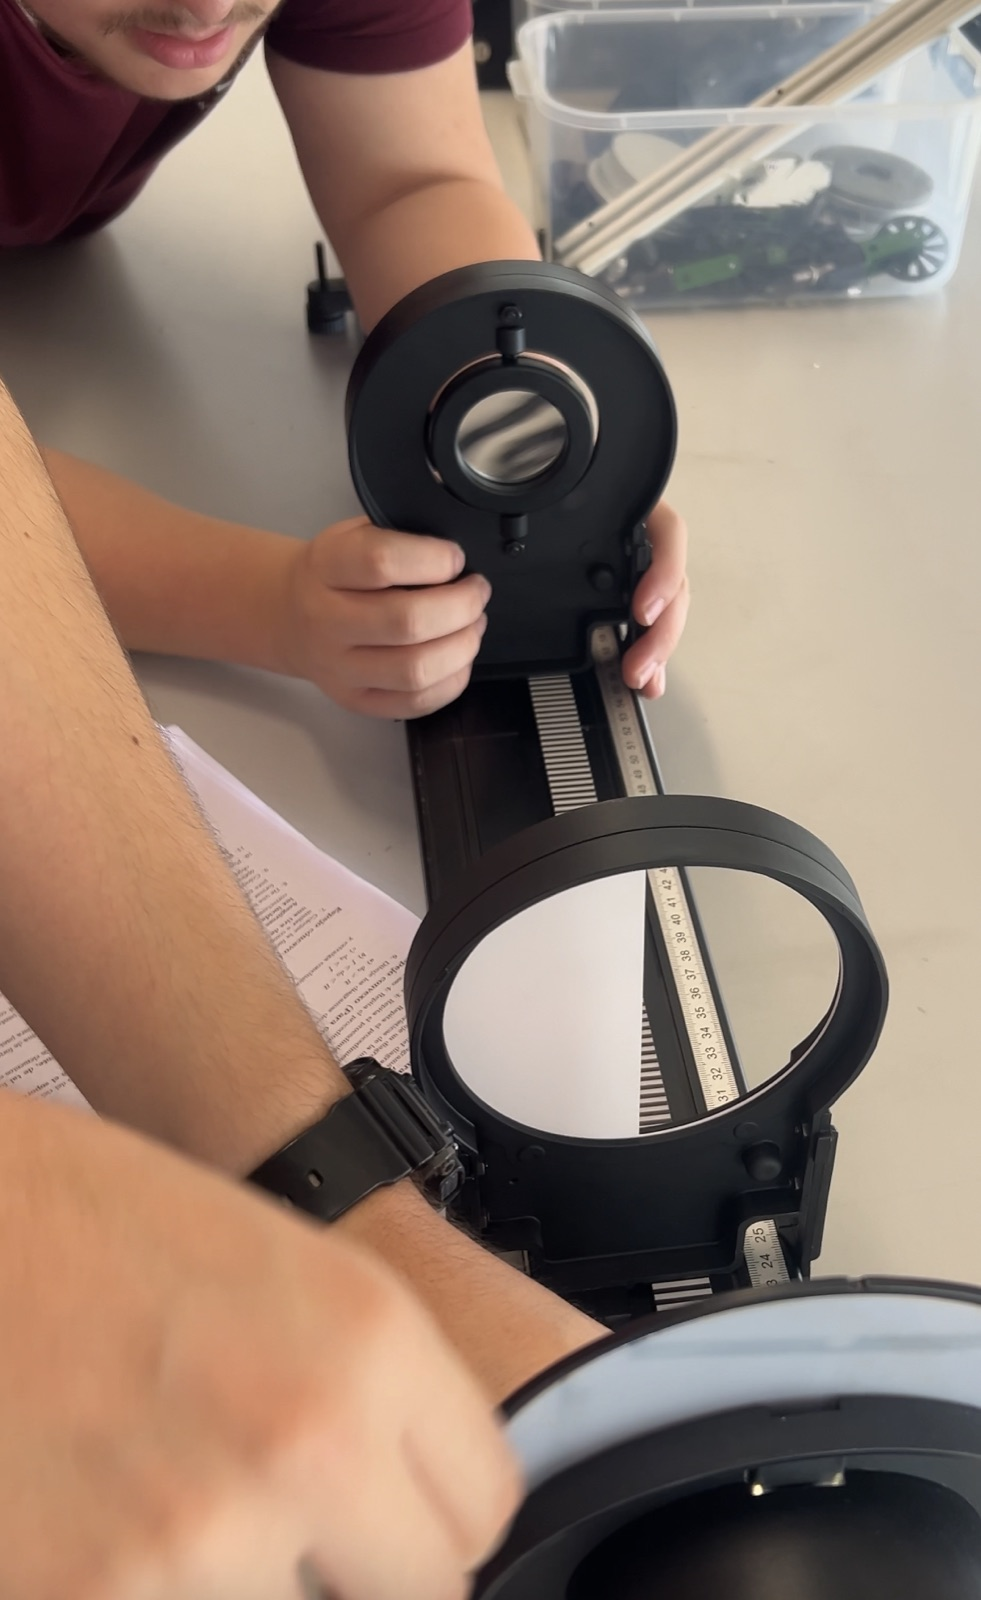
\includegraphics[height=8cm]{fotos/lab/convexo.jpg}
  \caption{Espejo convexo montado en el riel frente a la pantalla, al buscar la imagen.}
  \label{fig:convexo}
\end{figure}

% ===============================================================
\section{Resultados}

\subsection{Diagramas de rayos}

\begin{figure}[H]
  \centering
  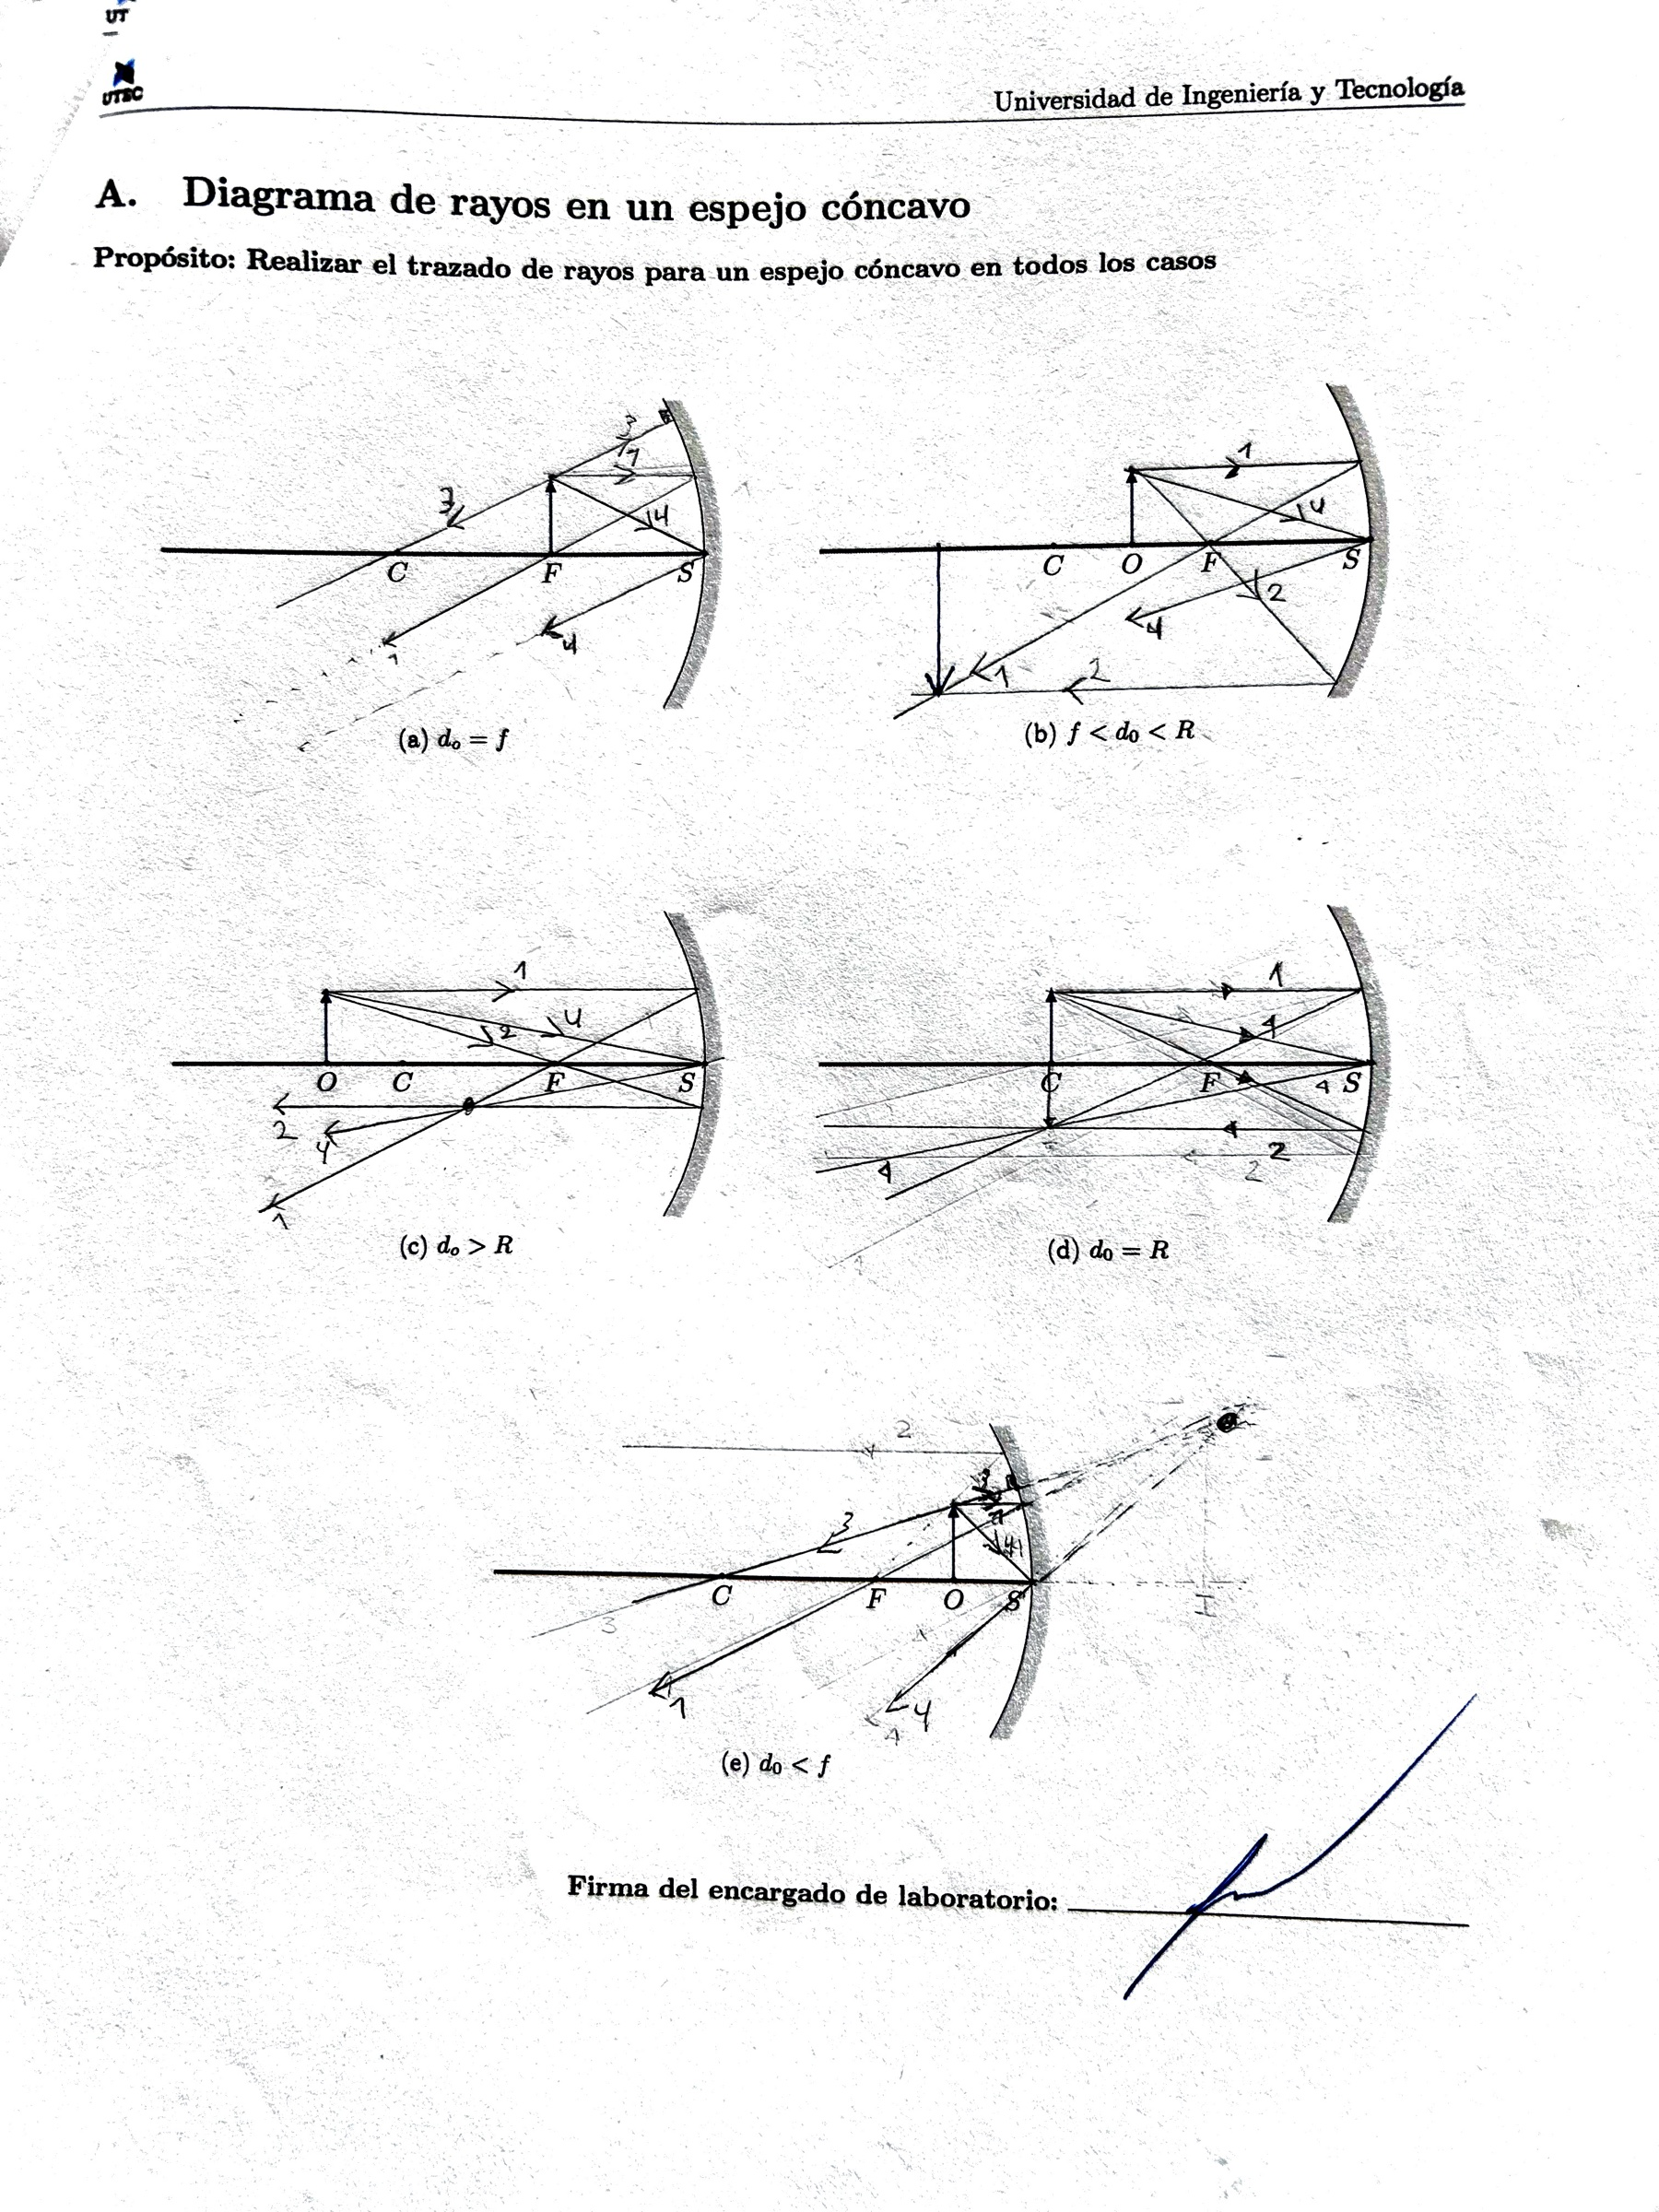
\includegraphics[width=0.82\linewidth]{fotos/escaneados/AnexoA.jpg}
  \caption{Apéndice A: diagramas de rayos en un espejo cóncavo (firmado por el encargado de laboratorio).}
\end{figure}

\begin{figure}[H]
  \centering
  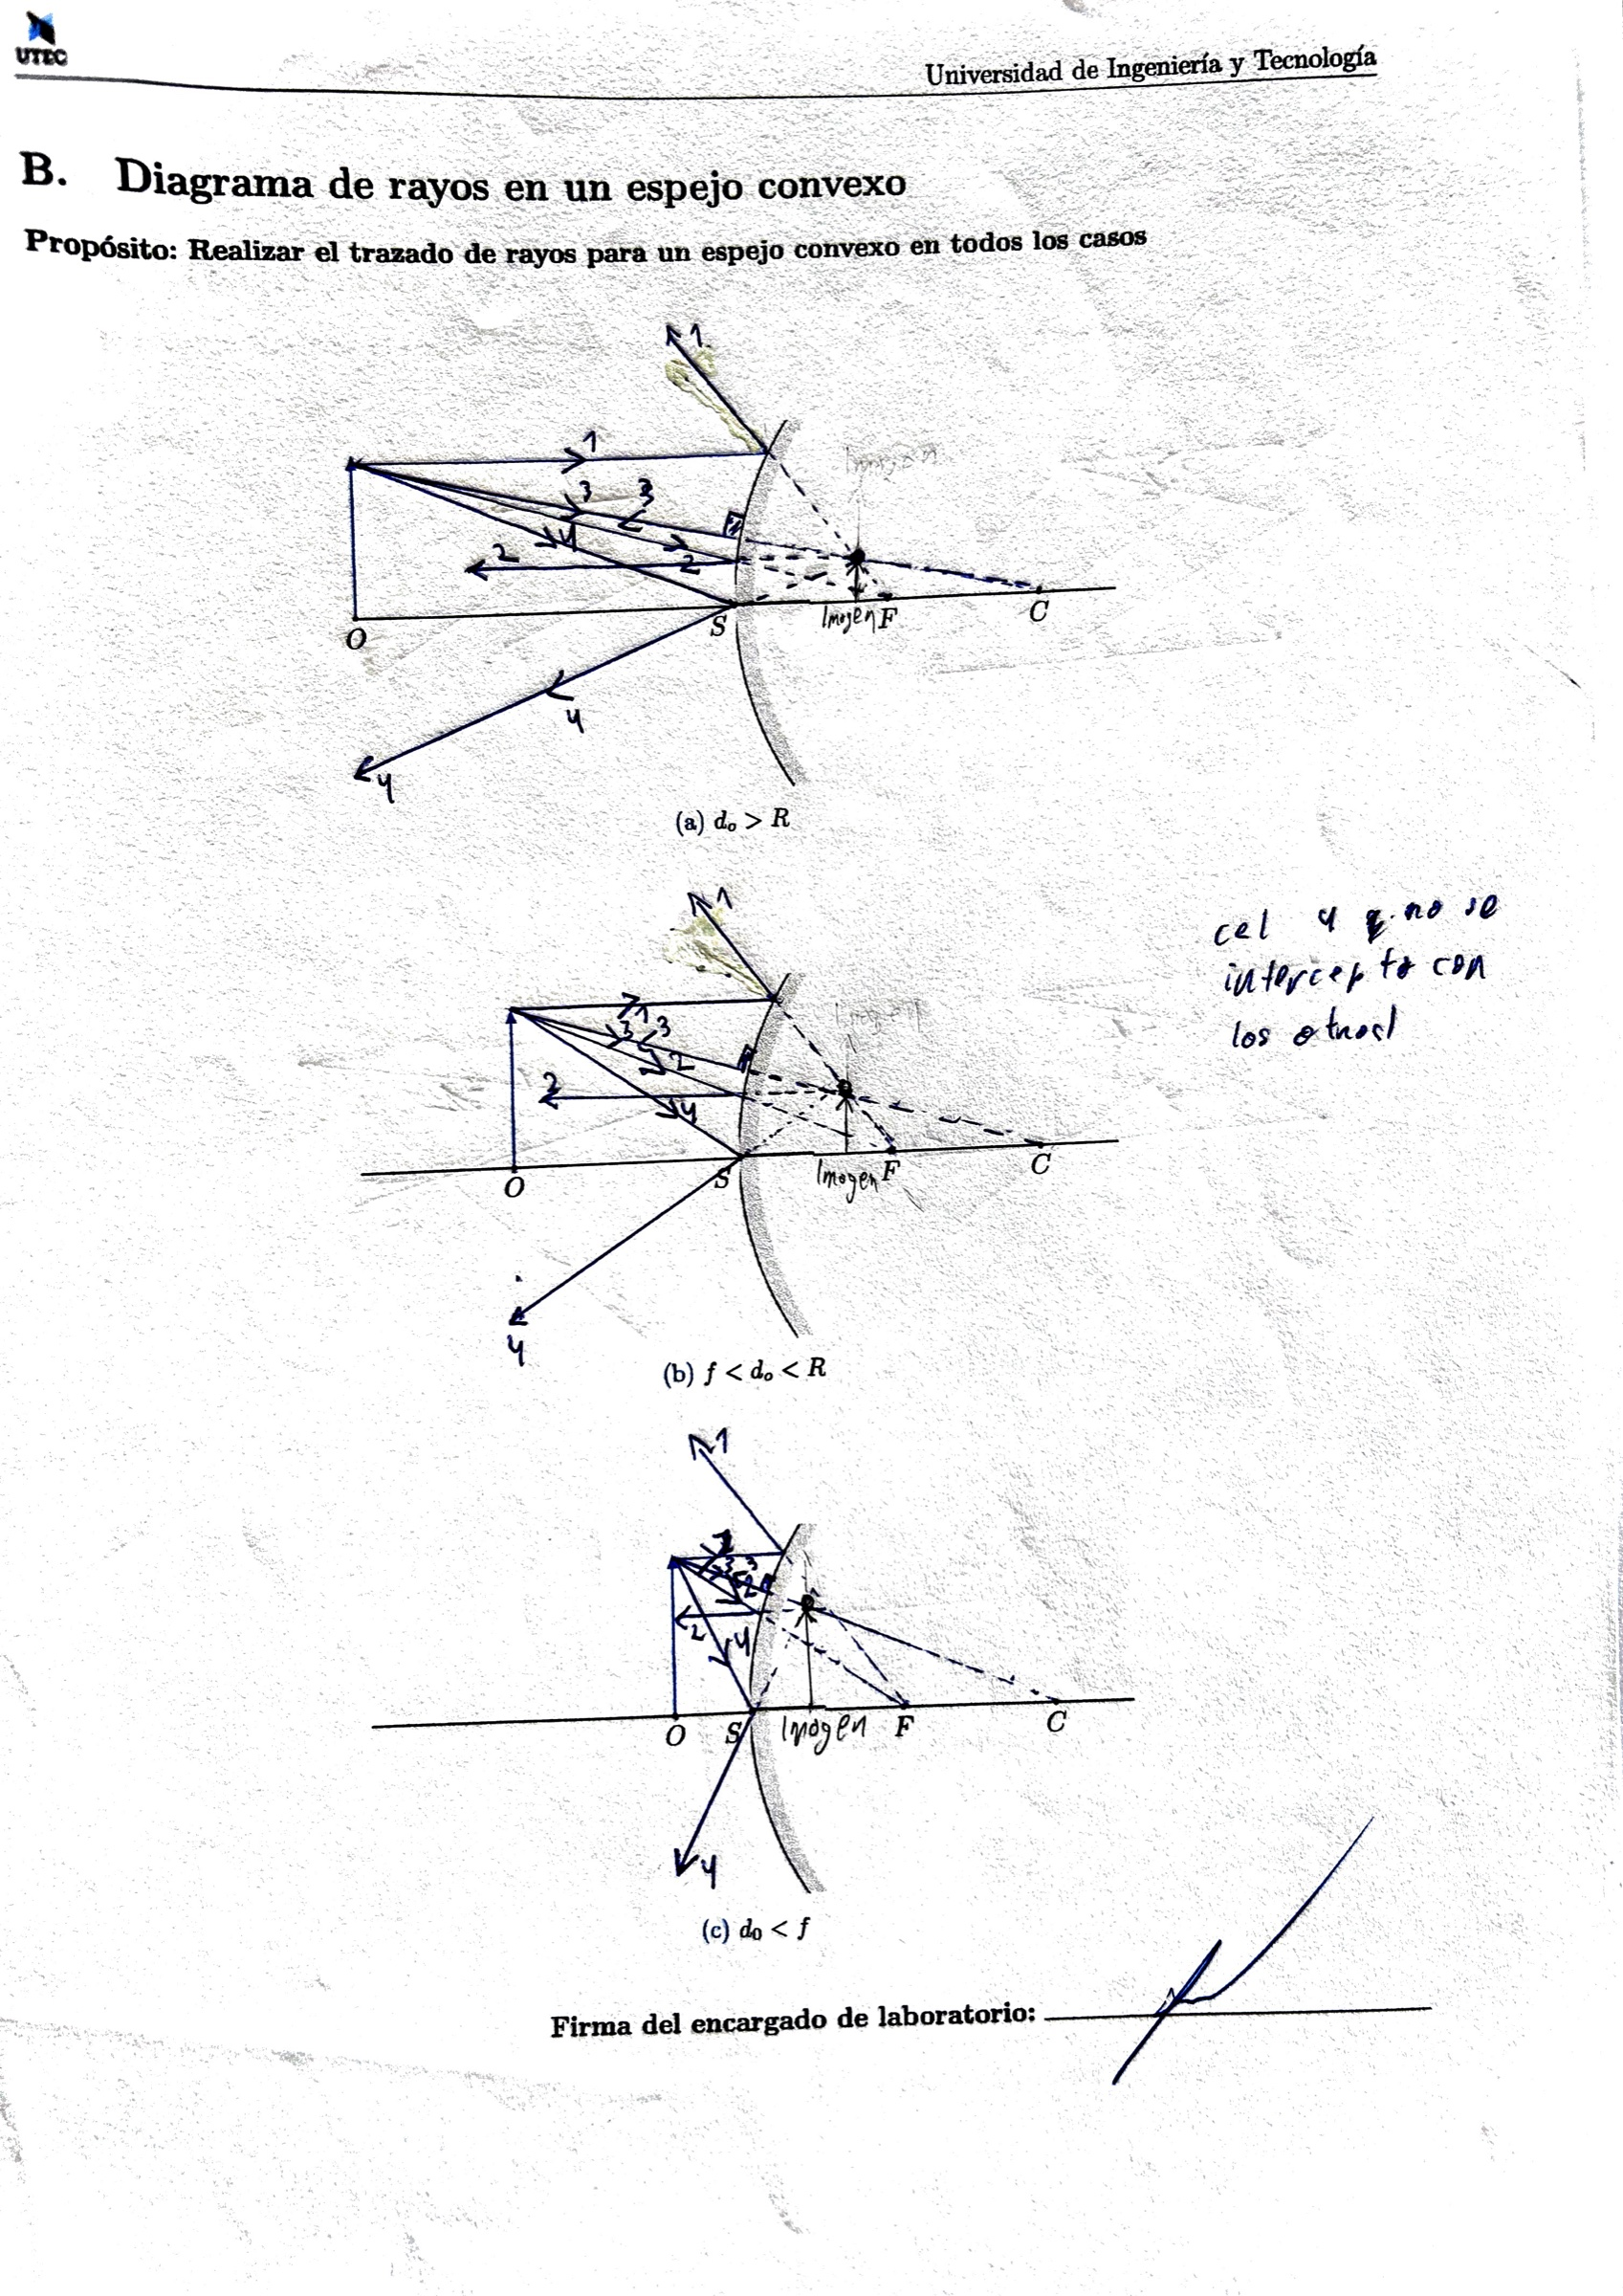
\includegraphics[width=0.82\linewidth]{fotos/escaneados/AnexoB.jpg}
  \caption{Apéndice B: diagramas de rayos en un espejo convexo (firmado por el encargado de laboratorio).}
\end{figure}

Los ocho diagramas reproducen la ubicación, el tipo, la orientación y el tamaño que predice la teoría. En el (a) del cóncavo ($d_o = f$), los rayos reflejados salen paralelos: la imagen está en el infinito ($1/d_i = 1/f - 1/f = 0$) y no puede proyectarse. En el (b) del convexo se anotó que el rayo 4 ``no se intercepta con los otros''; es un error del dibujo, pues por la ley de reflexión su prolongación debe pasar por la punta de la imagen virtual.

\subsection{Datos experimentales}

\begin{figure}[H]
  \centering
  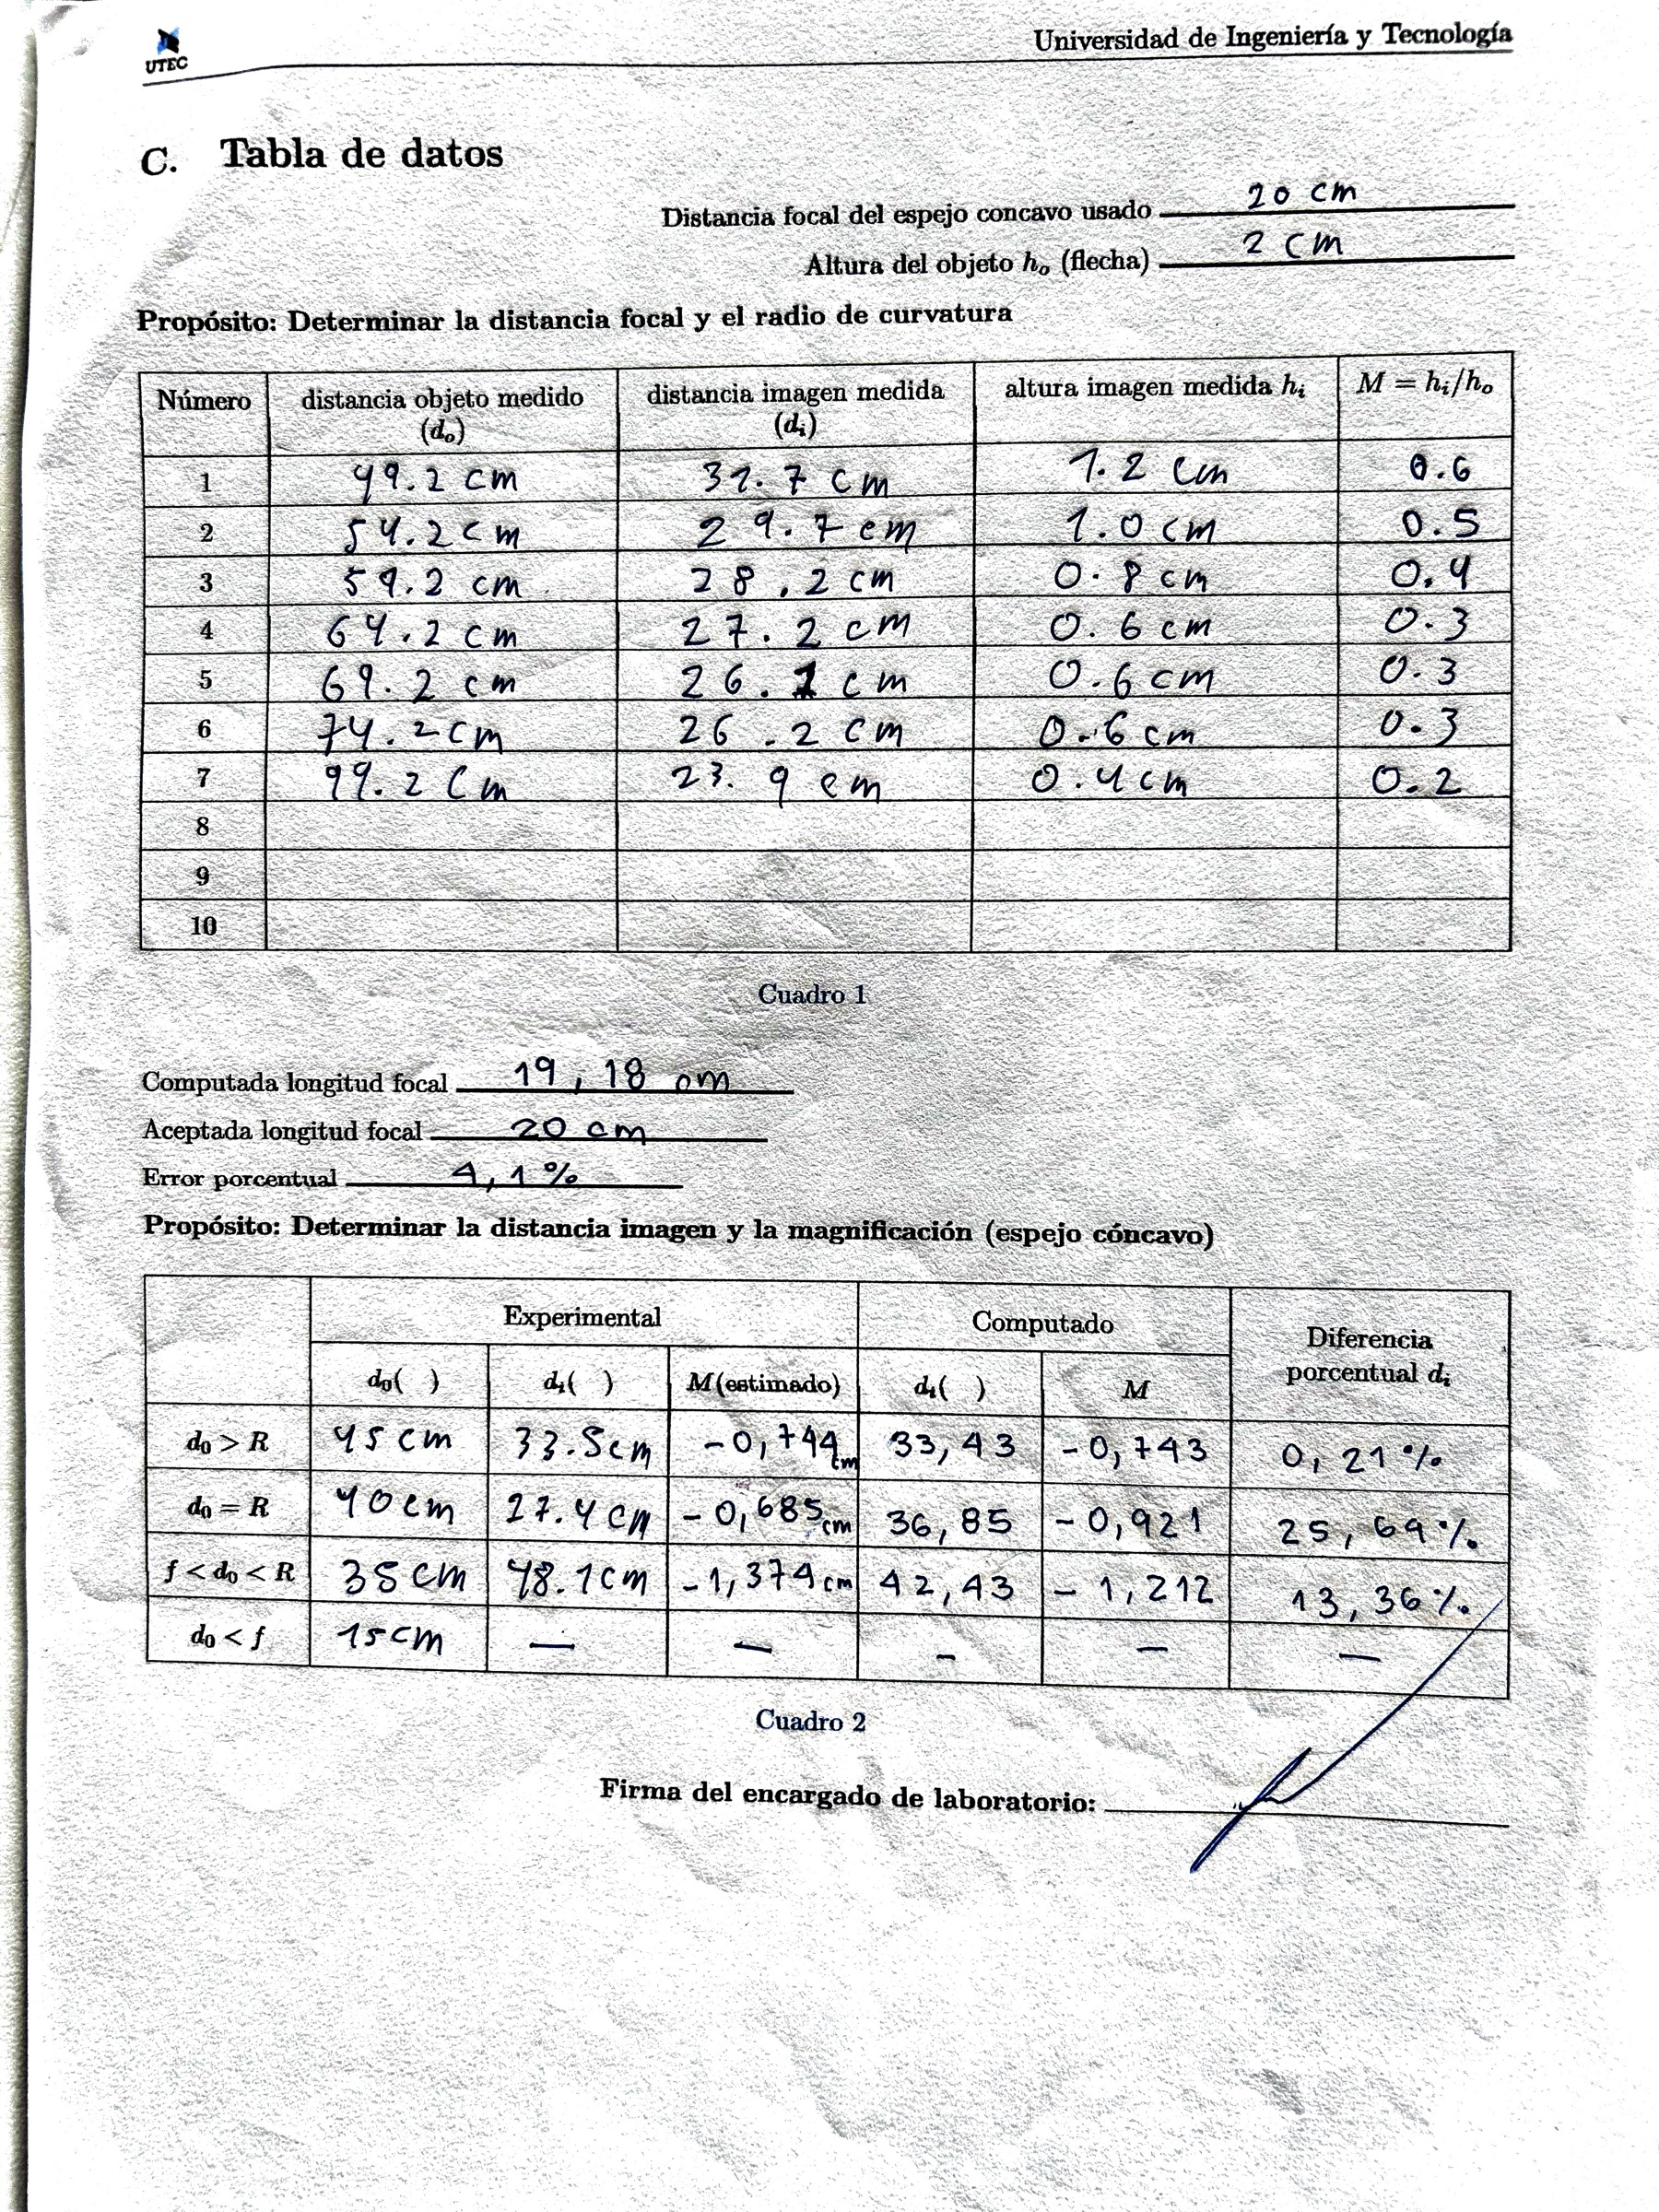
\includegraphics[width=0.82\linewidth]{fotos/escaneados/AnexoC.jpg}
  \caption{Apéndice C: tabla de datos (firmada por el encargado de laboratorio).}
\end{figure}

Valores nominales: $f_{\text{acep}} = 20$~cm y $h_o = 2.0$~cm. El Cuadro~\ref{tab:datos} transcribe la hoja y agrega columnas calculadas.

\begin{table}[H]
\centering
\begin{tabular}{ccccccc}
\toprule
\textbf{N.º} & $d_o$ (cm) & $d_i$ (cm) & $h_i$ (cm) & $M = h_i/h_o$ & $f_k = \left(\frac{1}{d_o}+\frac{1}{d_i}\right)^{-1}$ (cm) & $d_i/d_o$ \\
\midrule
1 & 49.2 & 31.7 & 1.2 & 0.6 & 19.28 & 0.644 \\
2 & 54.2 & 29.7 & 1.0 & 0.5 & 19.19 & 0.548 \\
3 & 59.2 & 28.2 & 0.8 & 0.4 & 19.10 & 0.476 \\
4 & 64.2 & 27.2 & 0.6 & 0.3 & 19.11 & 0.424 \\
5 & 69.2 & 26.1 & 0.6 & 0.3 & 18.95 & 0.377 \\
6 & 74.2 & 26.2 & 0.6 & 0.3 & 19.36 & 0.353 \\
7 & 99.2 & 23.9 & 0.4 & 0.2 & 19.26 & 0.241 \\
\bottomrule
\end{tabular}
\caption{Mediciones para determinar $f$ y $R$ ($M$, $f_k$ y $d_i/d_o$ son calculadas). $M$ se registró en magnitud; con signo es negativo (imagen invertida).}
\label{tab:datos}
\end{table}

\subsection{Distancia focal con la ecuación del espejo}

Para cada fila se aplicó la ecuación~\eqref{eq:espejo}. Por ejemplo, para la fila 1:
\[
  f_1 = \left(\frac{1}{49.2} + \frac{1}{31.7}\right)^{-1} = \left(0.02033 + 0.03155\right)^{-1} = 19.28 \text{ cm}
\]
Con los siete valores:
\[
  \bar f = 19.18 \text{ cm}, \qquad s_f = 0.14 \text{ cm}, \qquad \sigma_{\bar f} = \frac{s_f}{\sqrt{7}} = 0.05 \text{ cm}
\]
\[
  \boxed{f_{\text{comp}} = 19.18 \pm 0.05 \text{ cm}} \qquad R = 2f = 38.36 \pm 0.10 \text{ cm}
\]
\[
  \text{Error porcentual} = \frac{|f_{\text{comp}} - f_{\text{acep}}|}{f_{\text{acep}}}\times 100\text{\,\%} = \frac{|19.18 - 20|}{20}\times 100\text{\,\%} = 4.1\text{\,\%}
\]

\subsection{Distancia imagen y magnificación por casos}

Los valores computados usan $f = 19.18$~cm, $d_i = \dfrac{d_o f}{d_o - f}$ y $M = -\dfrac{d_i}{d_o}$; la diferencia porcentual es $\dfrac{|d_{i,\text{exp}} - d_{i,\text{comp}}|}{d_{i,\text{comp}}}\times 100\text{\,\%}$.

\begin{table}[H]
\centering
\small
\begin{tabular}{l ccc cc c}
\toprule
 & \multicolumn{3}{c}{\textbf{Experimental}} & \multicolumn{2}{c}{\textbf{Computado}} & \\
\cmidrule(lr){2-4}\cmidrule(lr){5-6}
\textbf{Caso} & $d_o$ (cm) & $d_i$ (cm) & $M$ (estimado) & $d_i$ (cm) & $M$ & \textbf{Dif.\ \% $d_i$} \\
\midrule
$d_o > R$ & 45 & 33.5 & $-0.744$ & 33.43 & $-0.743$ & 0.21\,\% \\
$d_o = R$ & 40 & 27.4 & $-0.685$ & 36.85 & $-0.921$ & 25.64\,\% \\
$f < d_o < R$ & 35 & 48.1 & $-1.374$ & 42.43 & $-1.212$ & 13.36\,\% \\
$d_o < f$ & 15 & \multicolumn{2}{c}{No se formó imagen} & $-68.83$ (virtual) & $+4.59$ & -- \\
\bottomrule
\end{tabular}
\caption{Distancia imagen y magnificación para el espejo cóncavo.}
\label{tab:casos}
\end{table}

\noindent Ejemplo de cálculo ($d_o > R$):
\[
  d_i = \frac{45 \times 19.18}{45 - 19.18} = \frac{863.1}{25.82} = 33.43 \text{ cm}, \quad M = -\frac{33.43}{45} = -0.743,
\]
\[
  \frac{|33.5 - 33.43|}{33.43}\times100\text{\,\%} = 0.21\text{\,\%}
\]
Para $d_o < f$: $d_i = \dfrac{15 \times 19.18}{15 - 19.18} = -68.83$~cm (imagen \textbf{virtual}) y $M = +4.59$ (\textbf{derecha y ampliada}).


\subsection{Espejo convexo}
\label{sec:convexo}
Con el objeto a una distancia arbitraria, la pantalla no mostró imagen en ninguna posición del riel (Figura~\ref{fig:convexo}): la imagen es \textbf{virtual}. Mirando el espejo sí se ve (Figura~\ref{fig:convexo_imagen}): la flecha y el entorno aparecen \textbf{derechos y reducidos}, con un campo visual amplio, como predicen el trazado de rayos (Apéndice B) y la ecuación del espejo con $f < 0$.

\begin{figure}[H]
  \centering
  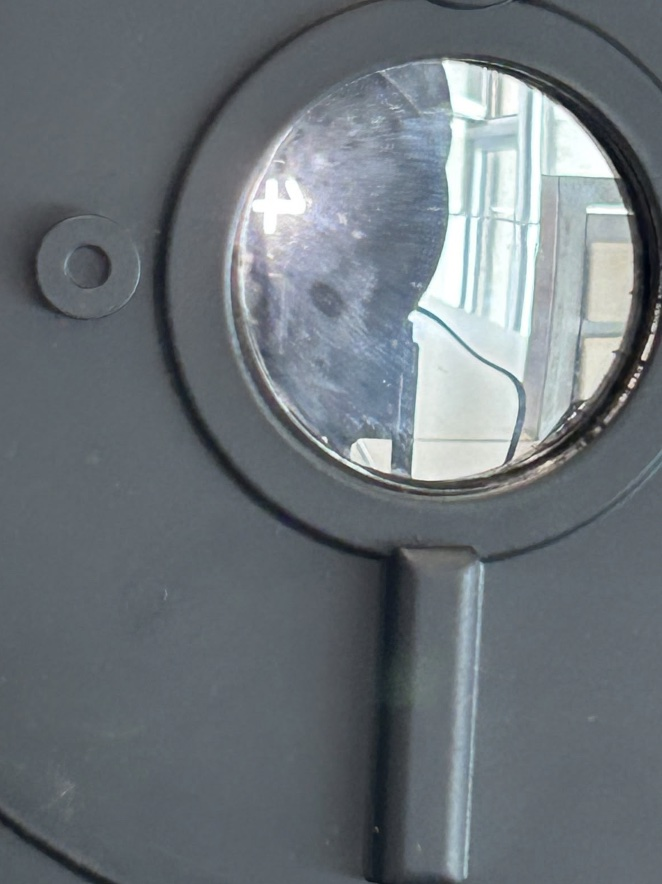
\includegraphics[height=7.5cm]{fotos/lab/convexo_imagen.jpg}
  \caption{Imagen vista en el espejo convexo: la flecha de la fuente (arriba a la izquierda) y el entorno aparecen derechos y reducidos. Esta imagen no puede proyectarse en la pantalla.}
  \label{fig:convexo_imagen}
\end{figure}


% ===============================================================
\section{Análisis de datos}
\label{sec:analisis}

\subsection{Magnificación en función de la distancia imagen}

\begin{figure}[H]
  \centering
  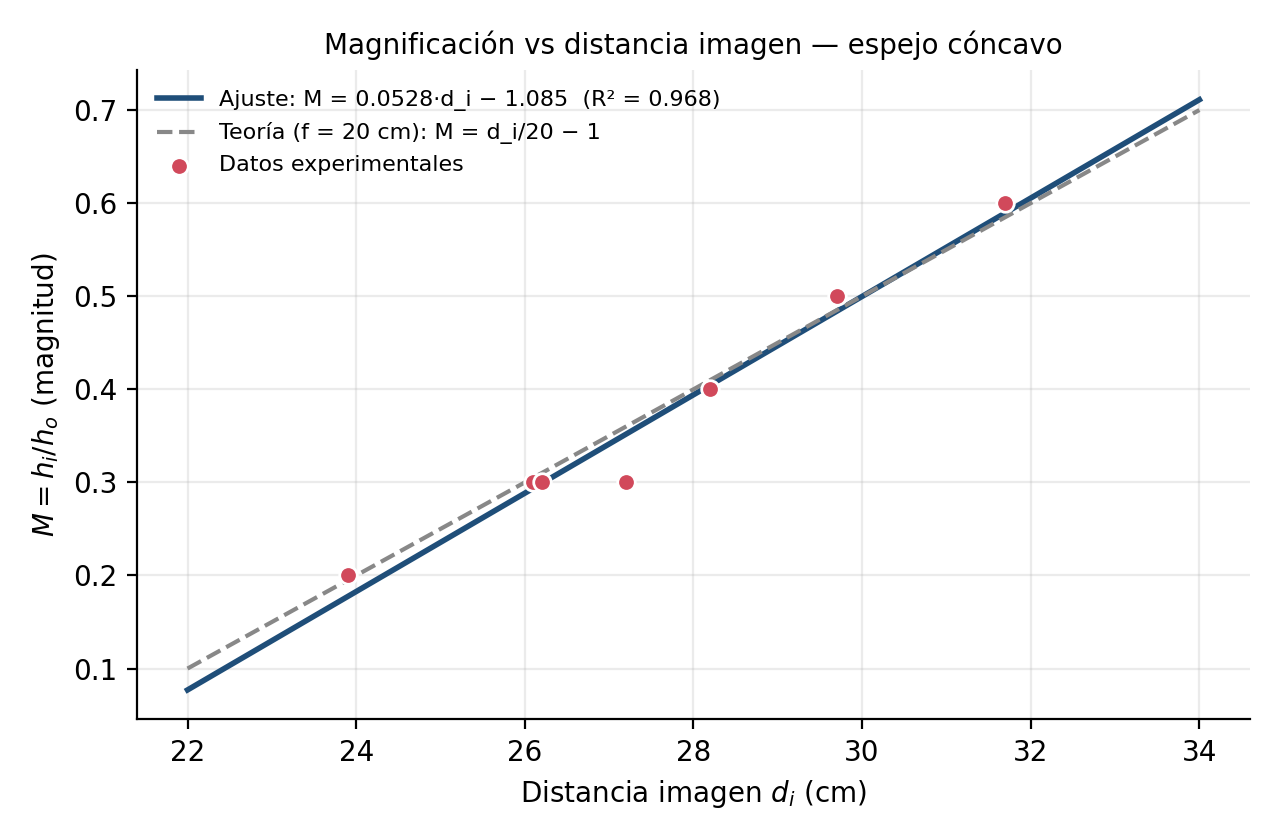
\includegraphics[width=0.8\linewidth]{figuras/grafico_M_vs_di.png}
  \caption{$M = h_i/h_o$ en función de $d_i$ (Cuadro~\ref{tab:datos}), con el ajuste lineal y la recta teórica para $f = 20$~cm.}
  \label{fig:ajuste}
\end{figure}

\paragraph{Resultado esperado.} Por la ecuación~\eqref{eq:lineal}, $|M|$ crece linealmente con $d_i$, con pendiente $1/f$ e intercepto $-1$: mientras más cerca del foco está el objeto, más lejos y más grande es la imagen. Los datos siguen esa tendencia (Figura~\ref{fig:ajuste}).

\paragraph{Ajuste.} Por mínimos cuadrados, $|M| = a\,d_i + b$ con
\[
  a = 0.0528 \pm 0.0043 \ \text{cm}^{-1}, \qquad b = -1.09 \pm 0.12, \qquad R^2 = 0.968
\]
\[
  \boxed{|M| = 0.0528\,d_i - 1.085} \qquad \left(\text{con signo: } M = -0.0528\,d_i + 1.085\right)
\]
El intercepto es compatible con $-1$ y el modelo explica el 96.8\,\% de la variación de $M$.

\paragraph{Distancia focal y radio de curvatura.}
\[
  f = \frac{1}{a} = 18.9 \pm 1.5 \text{ cm}, \qquad R = 2f = 37.8 \pm 3.1 \text{ cm}
\]
con $\sigma_f = \sigma_a/a^2$: error de 5.4\,\%, con 20~cm dentro de la incertidumbre. El ajuste es lineal porque lo exige la ecuación~\eqref{eq:lineal}. Su incertidumbre supera la del promedio porque $h_i$ (0.4 a 1.2~cm) se midió con regla, con errores relativos de 10 a 25\,\% (p.\ ej., el punto $d_i = 27.2$~cm, $M = 0.3$ se aleja de la recta).

\subsection{Distancia focal con las inversas de las distancias}
\label{sec:inversas}

Por la ecuación~\eqref{eq:inversas}, $1/d_o$ vs $1/d_i$ es una recta de pendiente $-1$ que corta el eje vertical en $1/f$. El Cuadro~\ref{tab:inversas} da las inversas del Cuadro~\ref{tab:datos}.

\begin{table}[H]
\centering
\begin{tabular}{ccccc}
\toprule
\textbf{N.º} & $d_o$ (cm) & $d_i$ (cm) & $1/d_o$ (cm$^{-1}$) & $1/d_i$ (cm$^{-1}$) \\
\midrule
1 & 49.2 & 31.7 & 0.02033 & 0.03155 \\
2 & 54.2 & 29.7 & 0.01845 & 0.03367 \\
3 & 59.2 & 28.2 & 0.01689 & 0.03546 \\
4 & 64.2 & 27.2 & 0.01558 & 0.03676 \\
5 & 69.2 & 26.1 & 0.01445 & 0.03831 \\
6 & 74.2 & 26.2 & 0.01348 & 0.03817 \\
7 & 99.2 & 23.9 & 0.01008 & 0.04184 \\
\bottomrule
\end{tabular}
\caption{Inversas de las distancias objeto e imagen.}
\label{tab:inversas}
\end{table}

\begin{figure}[H]
  \centering
  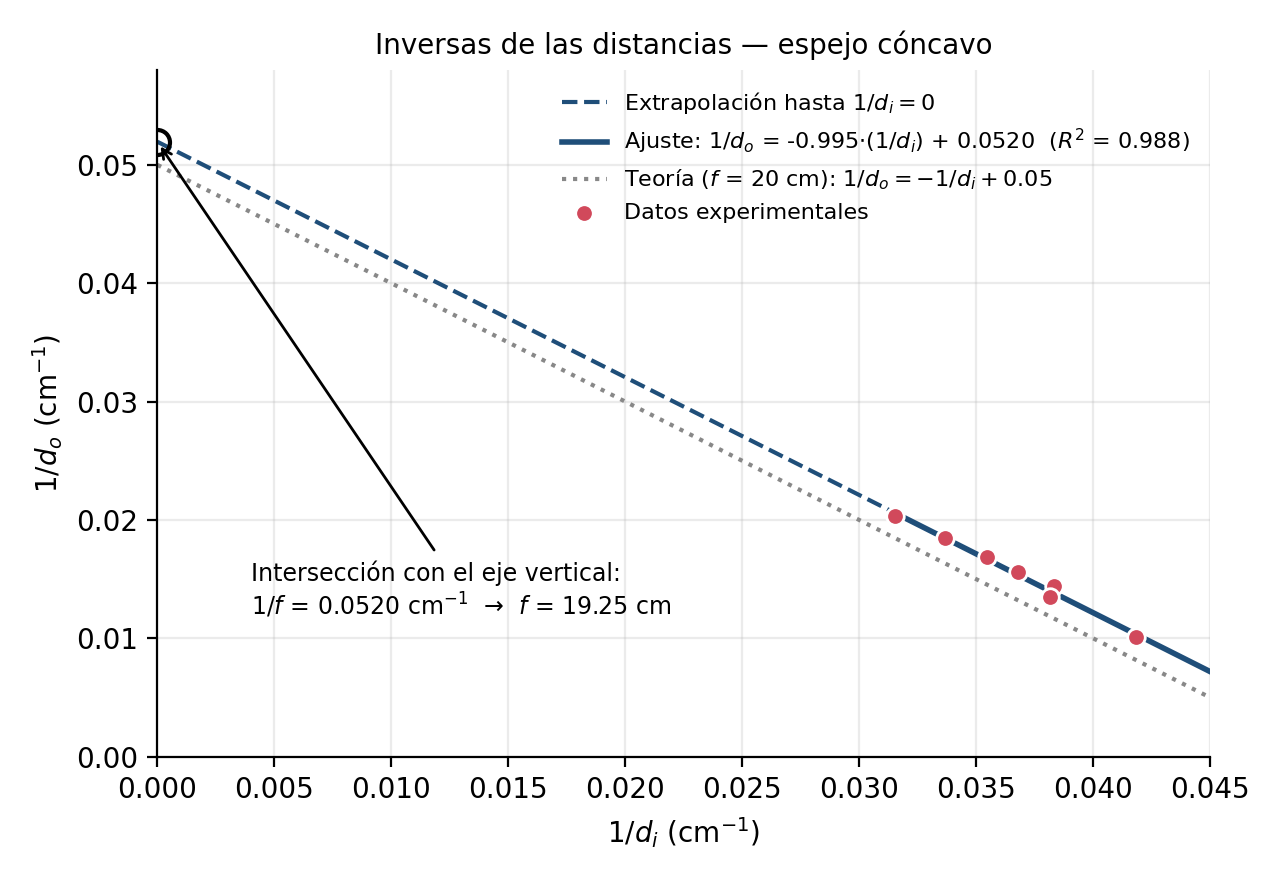
\includegraphics[width=0.8\linewidth]{figuras/grafico_inversas.png}
  \caption{$1/d_o$ en función de $1/d_i$, con el ajuste lineal y la recta teórica para $f = 20$~cm. El ajuste se prolonga hasta $1/d_i = 0$, donde su intersección con el eje vertical es $1/f$.}
  \label{fig:inversas}
\end{figure}

\paragraph{Ajuste.} Por mínimos cuadrados, $1/d_o = m\,(1/d_i) + b$ con
\[
  m = -0.995 \pm 0.050, \qquad b = 0.05195 \pm 0.00182 \ \text{cm}^{-1}, \qquad R^2 = 0.988
\]
y de la intersección con el eje vertical:
\[
  f = \frac{1}{b} = \boxed{19.25 \pm 0.67 \text{ cm}}, \qquad R = 2f = 38.5 \pm 1.3 \text{ cm}
\]
con $\sigma_f = \sigma_b/b^2$ y un error de 3.8\,\% respecto al valor nominal.

\paragraph{Comparación con la teoría.} Para $f = 20$~cm, la ecuación~\eqref{eq:inversas} predice la recta $1/d_o = -1/d_i + 0.0500$~cm$^{-1}$:
\begin{table}[H]
\centering
\begin{tabular}{lccc}
\toprule
\textbf{Parámetro} & \textbf{Teórico} & \textbf{Experimental} & \textbf{Diferencia} \\
\midrule
Pendiente $m$ & $-1$ & $-0.995 \pm 0.050$ & $0.1\,\sigma$ \\
Intersección vertical $1/f$ (cm$^{-1}$) & $0.0500$ & $0.0520 \pm 0.0018$ & $1.1\,\sigma$ \\
Intersección horizontal $1/f$ (cm$^{-1}$) & $0.0500$ & $0.0522$ & -- \\
\bottomrule
\end{tabular}
\caption{Parámetros de la recta de inversas: teoría vs.\ experimento.}
\label{tab:inversas_teoria}
\end{table}
\noindent Ambos parámetros coinciden con la teoría dentro de $2\sigma$. Por la simetría de la ecuación, la recta corta los dos ejes en $1/f$: $f = 19.25$~cm (vertical) y $19.15$~cm (horizontal).

\subsection{Comparación de los métodos}
El Cuadro~\ref{tab:metodos} reúne los tres valores de $f$ y $R$.

\begin{table}[H]
\centering
\begin{tabular}{lccc}
\toprule
\textbf{Método} & $f$ (cm) & $R$ (cm) & \textbf{Error} \\
\midrule
Ecuación del espejo (promedio de los $f_k$) & $19.18 \pm 0.05$ & $38.36 \pm 0.10$ & 4.1\,\% \\
Ajuste de $M$ vs $d_i$ & $18.9 \pm 1.5$ & $37.8 \pm 3.1$ & 5.4\,\% \\
Intersección de $1/d_o$ vs $1/d_i$ & $19.25 \pm 0.67$ & $38.5 \pm 1.3$ & 3.8\,\% \\
\bottomrule
\end{tabular}
\caption{Distancia focal y radio de curvatura según cada método (valor nominal: $f = 20$~cm).}
\label{tab:metodos}
\end{table}

\subsection{El caso extremo $d_o = 99.2$~cm}
\label{sec:extremo}
El séptimo punto se tomó lejos a propósito. Si $d_o \gg f$, la imagen se forma cerca del foco y $|M| \to 0$: aquí se midieron la menor $d_i$ (23.9~cm) y el menor aumento ($|M| = 0.2$), y $f_7 = 19.26$~cm coincide con el resto, así que el modelo sigue valiendo. Además amplía el rango de $1/d_i$, lo que reduce $\sigma_m = s/\sqrt{\sum (x_k - \bar x)^2}$:

\begin{table}[H]
\centering
\begin{tabular}{lcc}
\toprule
\textbf{Ajuste de $1/d_o$ vs $1/d_i$} & \textbf{Pendiente $m$} & $f$ (cm) \\
\midrule
Sin el caso extremo (6 puntos) & $-0.951 \pm 0.070$ & $19.83 \pm 0.99$ \\
Con el caso extremo (7 puntos) & $-0.995 \pm 0.050$ & $19.25 \pm 0.67$ \\
\bottomrule
\end{tabular}
\caption{Efecto del caso extremo $d_o = 99.2$~cm en el ajuste de inversas.}
\end{table}
\noindent Con él, la pendiente se acerca a $-1$ y las incertidumbres de $m$ y $f$ bajan cerca de un 30\,\%.

\subsection{Características de la imagen vs.\ trazado de rayos}
\label{sec:comparacion}

\begin{table}[H]
\centering
\small
\begin{tabularx}{\linewidth}{lXXl}
\toprule
\textbf{Caso} & \textbf{Experimental} & \textbf{Trazado de rayos} & \textbf{¿Coincide?} \\
\midrule
$d_o > R$ (45 cm) & Real (se proyectó); invertida y reducida según $M = -0.744$ & Real, invertida, reducida & Sí \\
$d_o = R$ (40 cm) & Real (se proyectó); invertida y reducida según $M = -0.685$ & Real, invertida, igual tamaño ($|M| = 1$) & No (descartado) \\
$f < d_o < R$ (35 cm) & Real (se proyectó); invertida y ampliada según $M = -1.374$ & Real, invertida, ampliada & Sí \\
$d_o < f$ (15 cm) & No se formó en la pantalla: virtual & Virtual, derecha, ampliada & Sí \\
Convexo & No se formó en la pantalla; vista en el espejo: virtual, derecha, reducida & Virtual, derecha, reducida & Sí \\
\bottomrule
\end{tabularx}
\caption{Resultados experimentales (Cuadro~\ref{tab:casos} y sección~\ref{sec:convexo}) vs.\ trazado de rayos. Que la imagen sea real se observó (se proyectó o no); la orientación y el tamaño en el cóncavo se deducen de $M = -d_i/d_o$, pues la hoja no los registra.}
\end{table}

Coinciden cuatro de los cinco casos. En $d_o = R$ la imagen debía ser del mismo tamaño, pero según $M$ resulta reducida y su $d_i$ es 25.6\,\% menor que la computada (secciones~\ref{sec:dR_grafica} y~\ref{sec:descarte}).

\subsection{El caso $d_o = R$ en la recta de inversas}
\label{sec:dR_grafica}
Se repitió el ajuste de inversas con y sin el par $(d_o, d_i) = (40, 27.4)$~cm.

\begin{figure}[H]
  \centering
  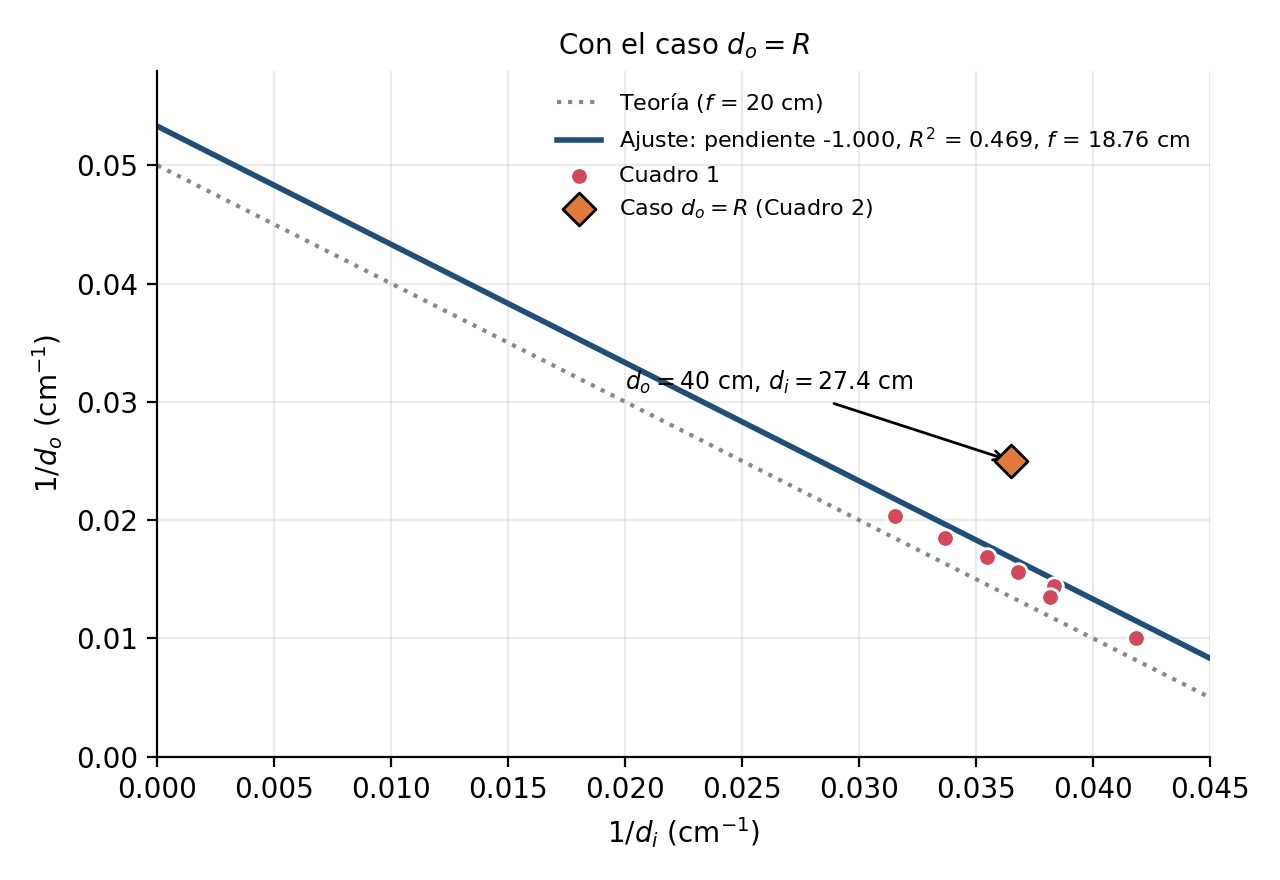
\includegraphics[width=0.78\linewidth]{figuras/inversas_con_dR.png}
  \caption{Recta de inversas \textbf{con} el caso $d_o = R$ (rombo naranja).}
  \label{fig:con_dR}
\end{figure}
\noindent Con el punto, la recta se desplaza y deja de pasar por los demás: $R^2$ cae a 0.469.

\begin{figure}[H]
  \centering
  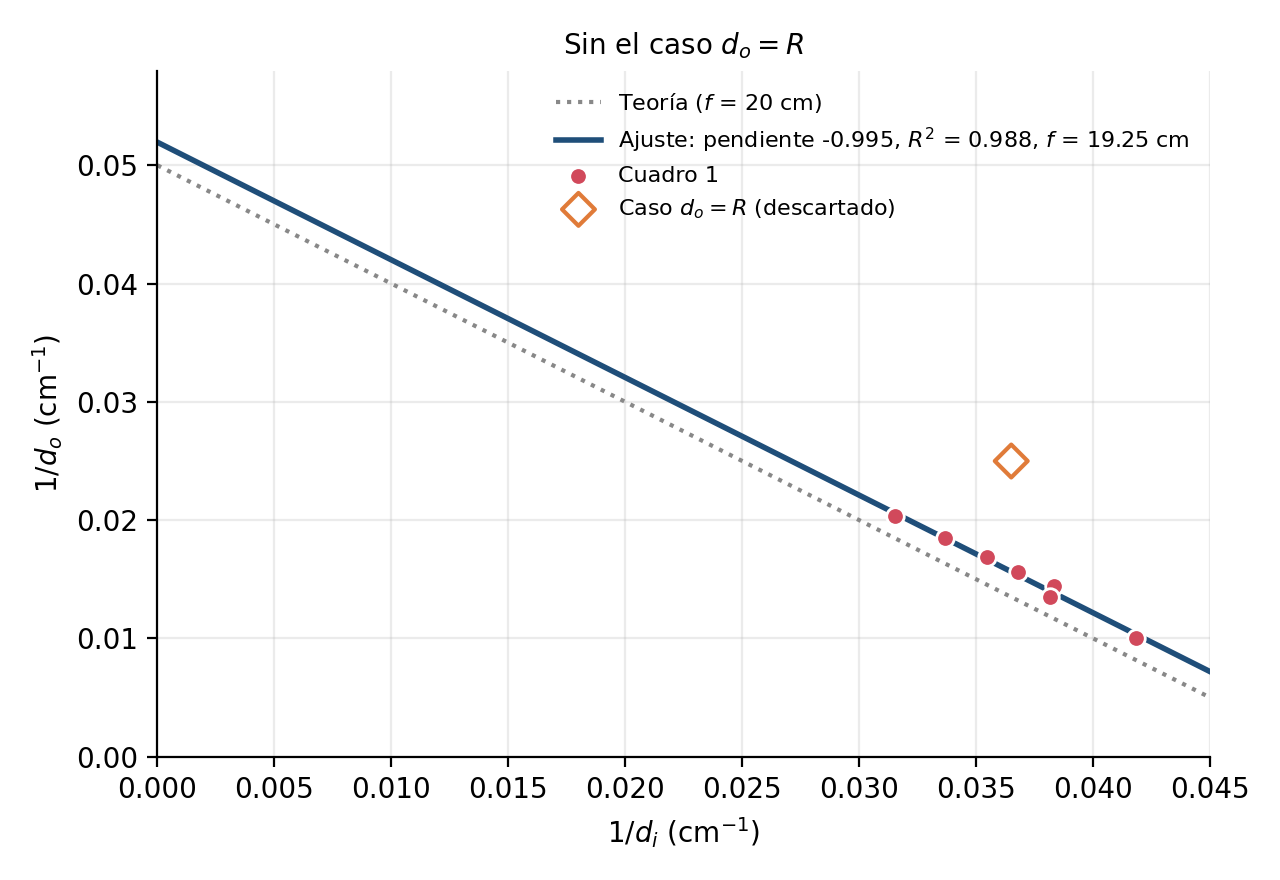
\includegraphics[width=0.78\linewidth]{figuras/inversas_sin_dR.png}
  \caption{Recta de inversas \textbf{sin} el caso $d_o = R$ (rombo vacío, descartado).}
  \label{fig:sin_dR}
\end{figure}
\noindent Sin él, la recta pasa por los siete puntos ($R^2 = 0.988$) y es paralela a la teórica; el rombo queda a unas 23 desviaciones típicas de ella (0.0094 frente a 0.0004~cm$^{-1}$).

\begin{table}[H]
\centering
\begin{tabular}{lcccc}
\toprule
\textbf{Ajuste de $1/d_o$ vs $1/d_i$} & \textbf{Pendiente} & $R^2$ & $f$ (cm) & \textbf{Error} \\
\midrule
Con el caso $d_o = R$ (8 puntos) & $-1.00 \pm 0.43$ & 0.469 & $18.8 \pm 5.6$ & 6.2\,\% \\
Sin el caso $d_o = R$ (7 puntos) & $-0.995 \pm 0.050$ & 0.988 & $19.25 \pm 0.67$ & 3.8\,\% \\
\bottomrule
\end{tabular}
\caption{Efecto del caso $d_o = R$ en el ajuste de inversas.}
\label{tab:descarte}
\end{table}
\noindent Con el punto, la incertidumbre de $f$ es más de 8 veces mayor (Cuadro~\ref{tab:descarte}); que la pendiente dé $-1.00$ es una coincidencia sin valor, dada su incertidumbre de $\pm 0.43$.

% ===============================================================
\section{Discusión}

\subsection{Espejo cóncavo vs.\ convexo}
El cóncavo ($f > 0$) forma imágenes reales e invertidas, proyectables, si $d_o > f$, y virtuales, derechas y ampliadas si $d_o < f$. En el convexo ($f < 0$), la ecuación~\eqref{eq:espejo} da $d_i < 0$ y $0 < M < 1$ para todo $d_o$: la imagen es siempre virtual, derecha y reducida.

Lo observado coincide con el trazado: con el cóncavo, la imagen se proyectó en los tres casos con $d_o > f$, donde los rayos reflejados se cortan delante del espejo (Apéndice A); con $d_o < f$ y con el convexo no se proyectó, y en los diagramas solo se cortan las prolongaciones, detrás del espejo. Que la imagen se proyecte o no es la forma experimental de distinguir ambos espejos.

\subsection{Interpretación de las rectas}
\label{sec:disc_inversas}
La recta de inversas (Figura~\ref{fig:inversas}) es casi paralela a la teórica (pendiente $-0.995$), pero está desplazada hacia arriba: los siete puntos quedan por encima de la teórica a una distancia casi constante (0.0017 a 0.0028~cm$^{-1}$). Esto indica que:
\begin{itemize}
  \item \textbf{La ecuación del espejo se cumple} en todo el rango medido (pendiente $-1$).
  \item \textbf{El error es sistemático:} uno aleatorio repartiría los puntos a ambos lados. Sumando un mismo desfase $\delta \approx 1.4$~cm a todas las $d_o$ y $d_i$ se recupera $f = 20$~cm. Podría deberse a que la marca leída en cada soporte no coincide con la flecha o el vértice del espejo (no verificado), y explicaría que los tres métodos den $f$ entre 3.8 y 5.4\,\% por debajo del nominal.
\end{itemize}

El método de inversas sitúa mejor $f$ que el de $M$ porque solo usa distancias, con errores relativos de 1 a 4\,\% (enfoque de $\sim$1~cm) frente a 10 a 25\,\% en $h_i$: mejor $R^2$ (0.988 frente a 0.968) y menor incertidumbre ($\pm 0.67$ frente a $\pm 1.5$~cm). Aun así, su incertidumbre supera la del promedio porque $1/f$ se extrapola desde $1/d_i \approx 0.032$--$0.042$~cm$^{-1}$ hasta 0, lo que amplifica el error de la pendiente. Fijando la pendiente en $-1$ se obtiene $f = 19.18$~cm, igual al promedio de los $f_k$.

\subsection{Descarte del caso $d_o = R$}
\label{sec:descarte}
El par $d_o = 40$~cm, $d_i = 27.4$~cm se conserva en el Cuadro~\ref{tab:casos} tal como fue firmado, pero no se usa en la interpretación:
\begin{enumerate}
  \item \textbf{Contradice las demás mediciones.} Para $d_o > f$, la imagen se aleja cuando el objeto se acerca:
  \[
    \frac{\mathrm{d}d_i}{\mathrm{d}d_o} = -\frac{f^2}{(d_o - f)^2} < 0 .
  \]
  A 49.2~cm la imagen se formó a 31.7~cm, así que a 40~cm debía formarse más lejos, no a 27.4~cm; ningún $f$ satisface ambos pares.
  \item \textbf{Es atípico.} Se aleja de la recta unas 23 desviaciones típicas (Figuras~\ref{fig:con_dR} y~\ref{fig:sin_dR}), y su diferencia con el valor computado (9.4~cm) es unas nueve veces la incertidumbre de enfoque ($\sim$1~cm).
  \item \textbf{Posible causa física.} En $d_o = R$ la imagen se forma sobre la fuente, donde la pantalla taparía la luz; quizá se colocó más adelante, sobre una imagen algo borrosa, lo que daría una $d_i$ menor (la hoja no registra la posición de la pantalla). También podría ser un error de registro: 27.4~cm corresponde a $d_o \approx 64$~cm, casi igual a la fila 4 (64.2; 27.2~cm).
\end{enumerate}
Descartarlo no cambia ningún resultado: no interviene en el cálculo de $f$ ni en los ajustes.

El caso $f < d_o < R$ (13.36\,\%) se conserva: respeta la tendencia (es la mayor $d_i$) y coincide con el trazado. Su imagen debía formarse $\sim$7~cm detrás de la fuente y la $d_i$ medida (48.1~cm) la ubica a $\sim$13~cm; con la flecha en la marca de 8~cm, eso queda $\sim$5~cm antes del inicio de la escala del riel, y la hoja no registra cómo se ubicó la pantalla. Que la imagen quede detrás de la fuente podría explicar que la diferencia sea mayor que en $d_o > R$ (0.21\,\%).

\subsection{Fuentes de error}
\begin{enumerate}
  \item \textbf{Criterio de enfoque:} la imagen se ve nítida en un intervalo de $\sim$1~cm, y la posición elegida depende del observador.
  \item \textbf{Medición de $h_i$:} el grosor de las marcas de plumón y la resolución de la regla (1~mm) son grandes frente a imágenes de 0.4 a 1.2~cm.
  \item \textbf{Posición del vértice:} si la marca del soporte no coincide con el vértice, todas las distancias tienen el mismo desfase (sección~\ref{sec:disc_inversas}).
  \item \textbf{Imagen sobre o detrás de la fuente:} en $d_o = R$ la pantalla taparía la luz que va al espejo; en $f < d_o < R$ la fuente tapa parte de la luz reflejada.
  \item \textbf{Alineación y aberración esférica:} el espejo y la fuente no están perfectamente centrados en el eje, y no todos los rayos son paraxiales.
\end{enumerate}

\subsection{Observaciones}
\begin{itemize}
  \item En el caso extremo ($d_o = 99.2$~cm) la imagen mide solo 0.4~cm, lo que dificulta medir $h_i$; aun así, el punto sigue la tendencia del resto.
\end{itemize}

\subsection{Sugerencias}
\begin{itemize}
  \item Medir cada $d_i$ dos o tres veces, acercando y alejando la pantalla, y promediar.
  \item Medir $h_i$ con una pantalla milimetrada o fotografiando la pantalla junto a una regla, y usar un objeto más grande.
  \item Medir la posición real del vértice del espejo respecto a la marca del soporte y corregir las distancias.
  \item Para $d_o \le R$, inclinar ligeramente el espejo para que la imagen se forme al costado de la fuente.
  \item Tomar más puntos con el objeto lejos del espejo, para reducir la extrapolación en la recta de inversas.
\end{itemize}

\subsection{Reflexión adicional}
\begin{enumerate}
  \item \textbf{Ajuste restringido al modelo.} Fijando el intercepto de $M$ vs $d_i$ en $-1$, como exige la ecuación~\eqref{eq:lineal}, se obtiene $f = 20.1$~cm (0.5\,\%): la desviación del ajuste libre viene del ruido en $h_i$, no del modelo.
  \item \textbf{$M$ a partir de distancias.} Con $|M| = d_i/d_o$, el ajuste da $|M| = 0.0516\,d_i - 0.985$, $R^2 = 0.9945$ y $f = 19.4 \pm 0.6$~cm (3.1\,\%): las distancias son más confiables que las alturas.
  \item \textbf{Aplicaciones.} El espejo convexo se usa en retrovisores y en vigilancia porque su imagen virtual, derecha y reducida amplía el campo visual. El cóncavo se usa en linternas (fuente en $F$, haz reflejado paralelo) y en espejos de maquillaje ($d_o < f$, imagen derecha y ampliada).
\end{enumerate}

% ===============================================================
\section{Conclusiones}
\begin{enumerate}
  \item $f = 19.18 \pm 0.05$~cm (ecuación del espejo), $18.9 \pm 1.5$~cm (ajuste de $M$ vs $d_i$) y $19.25 \pm 0.67$~cm (recta de inversas), con errores de 4.1, 5.4 y 3.8\,\% respecto al nominal; $R \approx 38$~cm.
  \item La ecuación del espejo se cumple: $M$ es lineal en $d_i$ (intercepto compatible con $-1$) y la recta de inversas tiene pendiente $-0.995$. Los tres valores de $f$ quedan por debajo del nominal, lo que apunta a un error sistemático común en las distancias.
  \item Las imágenes coinciden con el trazado de rayos: reales e invertidas para $d_o > f$ (reducidas si $d_o > R$, ampliadas si $f < d_o < R$) y virtuales para $d_o < f$. El caso $d_o = R$ se descartó por contradecir las demás mediciones.
  \item La imagen del convexo es virtual, derecha y reducida: no se proyectó en ninguna posición, pero se vio en el espejo. Es la diferencia experimental clave entre ambos espejos.
\end{enumerate}

\end{document}
